% =============================================================================
% Title:        Failure Report
% Author:       Nathaniel Thomas
% Affiliation:  Texas A&M University, Department of Nuclear Engineering
% Email:        nathaniel@tamu.edu
% Date Created: 3/7/2026
% Version:      1.0
%
% Description:
%   A .tex source file describing the failures of the FLiNaK purifier.
%
% =============================================================================

\section{Failure Report}
\label{sec: failure report}

This section goes over the failure modes of the FLiNaK purifier. While the
purifier has worked for a number of runs, it has had a number of failure as
well. A few failures were due to operator error, while most failures were
due to inadequate heating during transfers. \par

% TODO: Ask Kyle for pictures and details on why he opened the scrubber line.
% also get the date.
An early failure was due to operator error. On [DATE], the purifier was heated
to operating temperature with salt loaded inside, before being sealed and cooled
down again. The cooling resulted in the gas inside the reaction chamber
reducing in pressure. Later on, the line going to the scrubber line was opened,
causing the caustic scrubber solution to be sucked into the reaction chamber.
Approximately \SI{5}{\kilo\gram} of salt was contaminated, and the reaction
chamber had to be opened for cleanup.
\par

Later on, the purifier was run successfully, and the salt transfer process
was partially successful. However, the transfer required some manual heating of
the uncovered portions of the transfer line, as a result of salt freezing.
Refer to \Cref{fig: purifier transfer tank} and
\Cref{fig: purifier reaction chamber} to see the unheated portions of the
transfer line. Heat was applied using a blowtorch and MAP gas to melt the salt
and facilitate transfer.
\par

\begin{figure}
  \centering
  \includegraphics[width=0.6\textwidth]{./assets/pictures/purifier
  transfer tank.jpg}
  \caption{Image of the unheated portion of the transfer line before heating.}
  \label{fig: purifier transfer tank}
\end{figure}

\begin{figure}
  \centering
  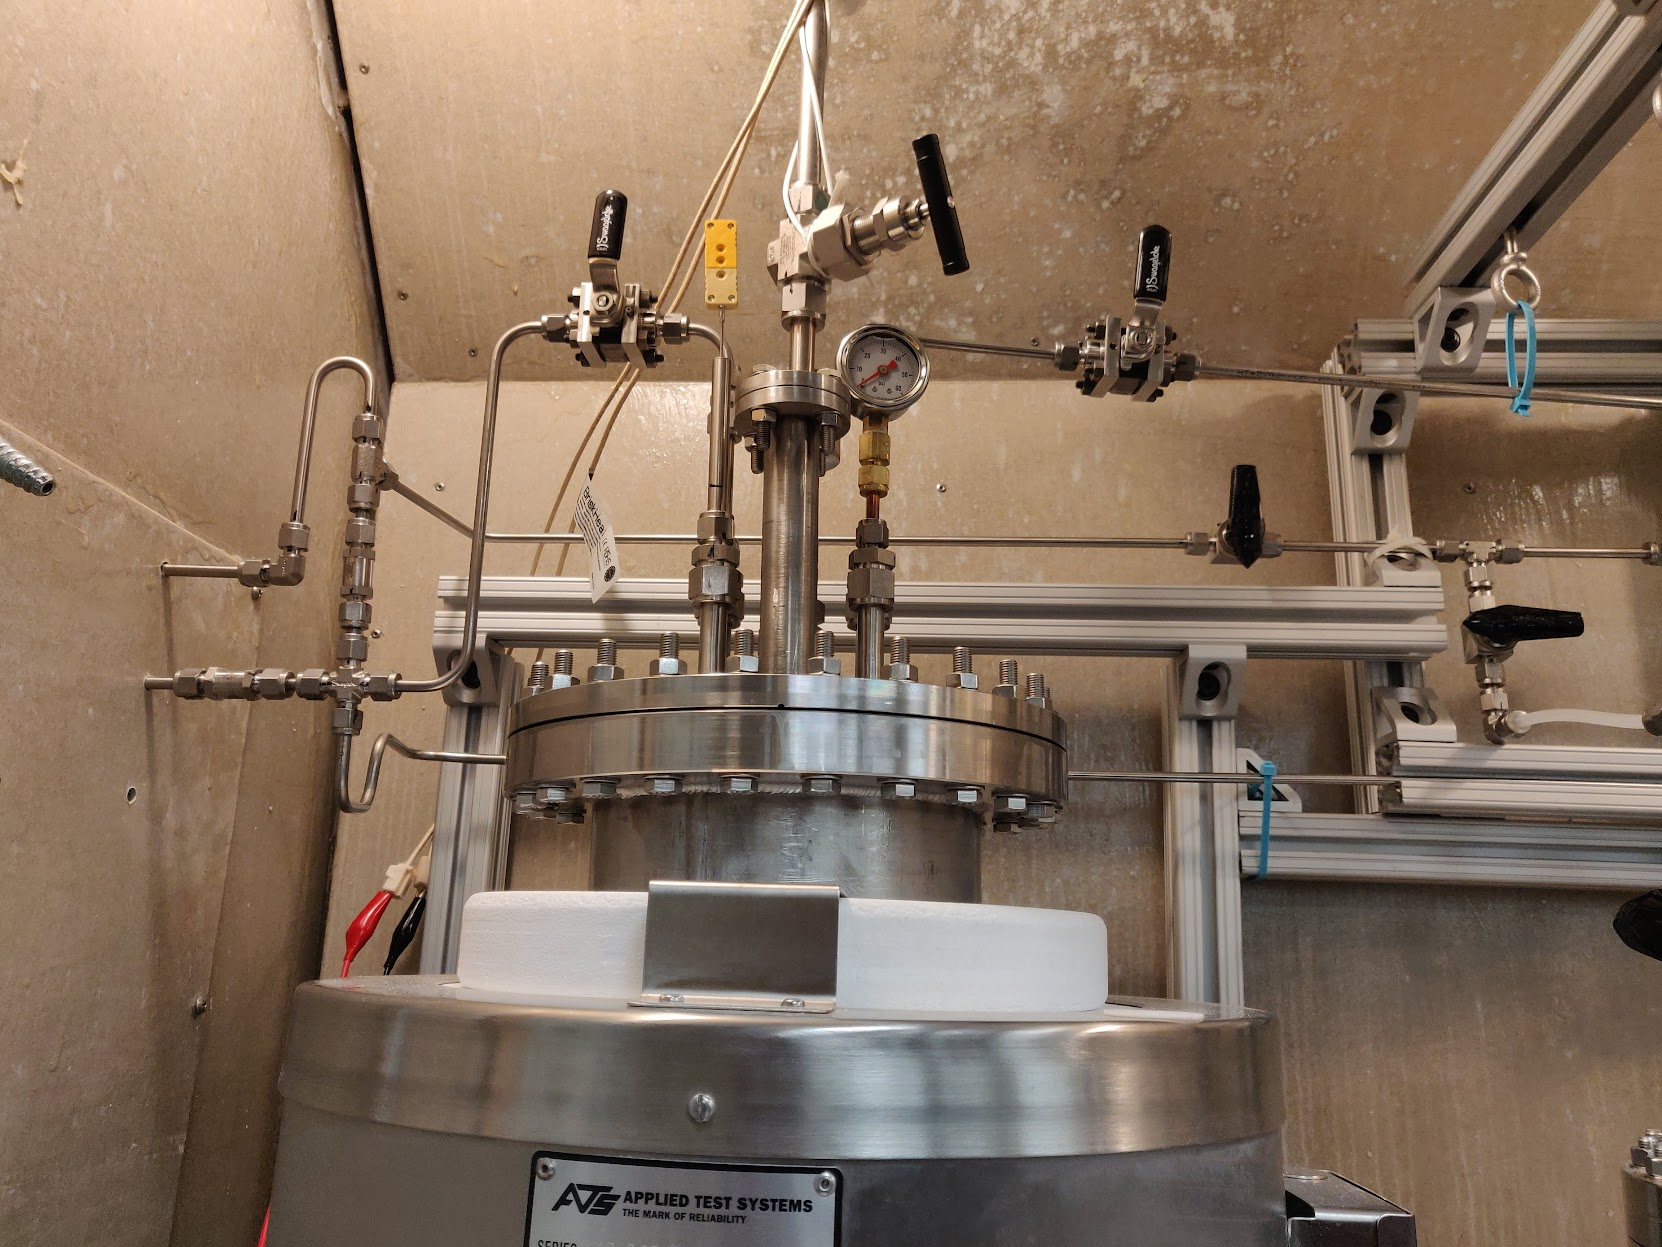
\includegraphics[width=0.6\textwidth]{
    ./assets/pictures/purifier reaction chamber.jpg
  }
  \caption{Image of the unheated portion of the reaction chamber line
  before heating.}
  \label{fig: purifier reaction chamber}
\end{figure}

Following purification, samples of the purified salt were removed from the
transfer tank and processed for ICPMS. The results of the ICPMS indicated
that most metallic impurities were reduced, but the concentration of
aluminum was increased. This was attributed to some of the alumina insulation
falling into the purifier while salt was being loaded. \par

% TODO: Ask Kyle for ICPMS data.
% TODO: Show combustion analyzer data
% TODO: Check the order of events here.

Following combustion analysis, it was found that hydrogen fluoride was not
being sparged through the FLiNaK due to the high oxygen content in the salt.
The flow controller connected to the hydrogen fluoride cylinder was found to
be non-functional. The controls for the flow controller was modified to work
with the LabView program and tested. It was then reattached and purification
was attempted again, but with hydrogen fluoride introduced to the
sparging gas. \par

% TODO: The order of events here is not clear. Clarify with Kyle.
However, it was found that the hydrogen fluoride was condensing in the
transparent polyfluorocarbon feed line to the controller. This was due
to the low boiling point of HF (\SI{67.1}{\celsius}). This resuhis,lted
in hydrogen fluoride liquid passing through the flow controller.
This damaged the flow controller and disabled it from opening. Because
of this, liquid HF accumulated in the feed line, and the liquid had to be
released into a KOH scrubbing solution. The flow controller was submerged in
the solution and was destroyed. \par

An Aalborg flow controller replaced the gas flow controller and was used to
conduct a successful hydrofluorination. The \ch{HF} cylinder was also
wrapped with
a cylinder heating band to encourage HF vaporization and reduce condensation.
Following this change, the \ch{HF} was successfully introduced to the system.
However, due to occasional liquid buildup, the supply (the HF cylinder) had to
be shut approximately every hour to allow HF to boil off and avoid flooding the
flow controller.
\par

% TODO: Based solely on my memory, confirm with pictures and Kyle.

Purification was successful and completed without incident. However, the
transfer stage of the purifier operation was not successful. Heating tape
was applied to the transfer line, including along the valves, but the heating
tape was not able to bring the transfer line above the melting point of
FLiNaK (\SI{462}{\celsius}). Because of this, FLiNaK was trapped in
the micron filter that was used to extract precipitated purification
products and froze. This prevented the transfer from succeeding. Images of the
clogged components can be seen in
\Cref{fig: transfer lid clog,fig:
  clogged needle valve front,fig:
  clogged needle valve back,fig:
fully clogged needle valve}. \par

\begin{figure}[H]
  \centering
  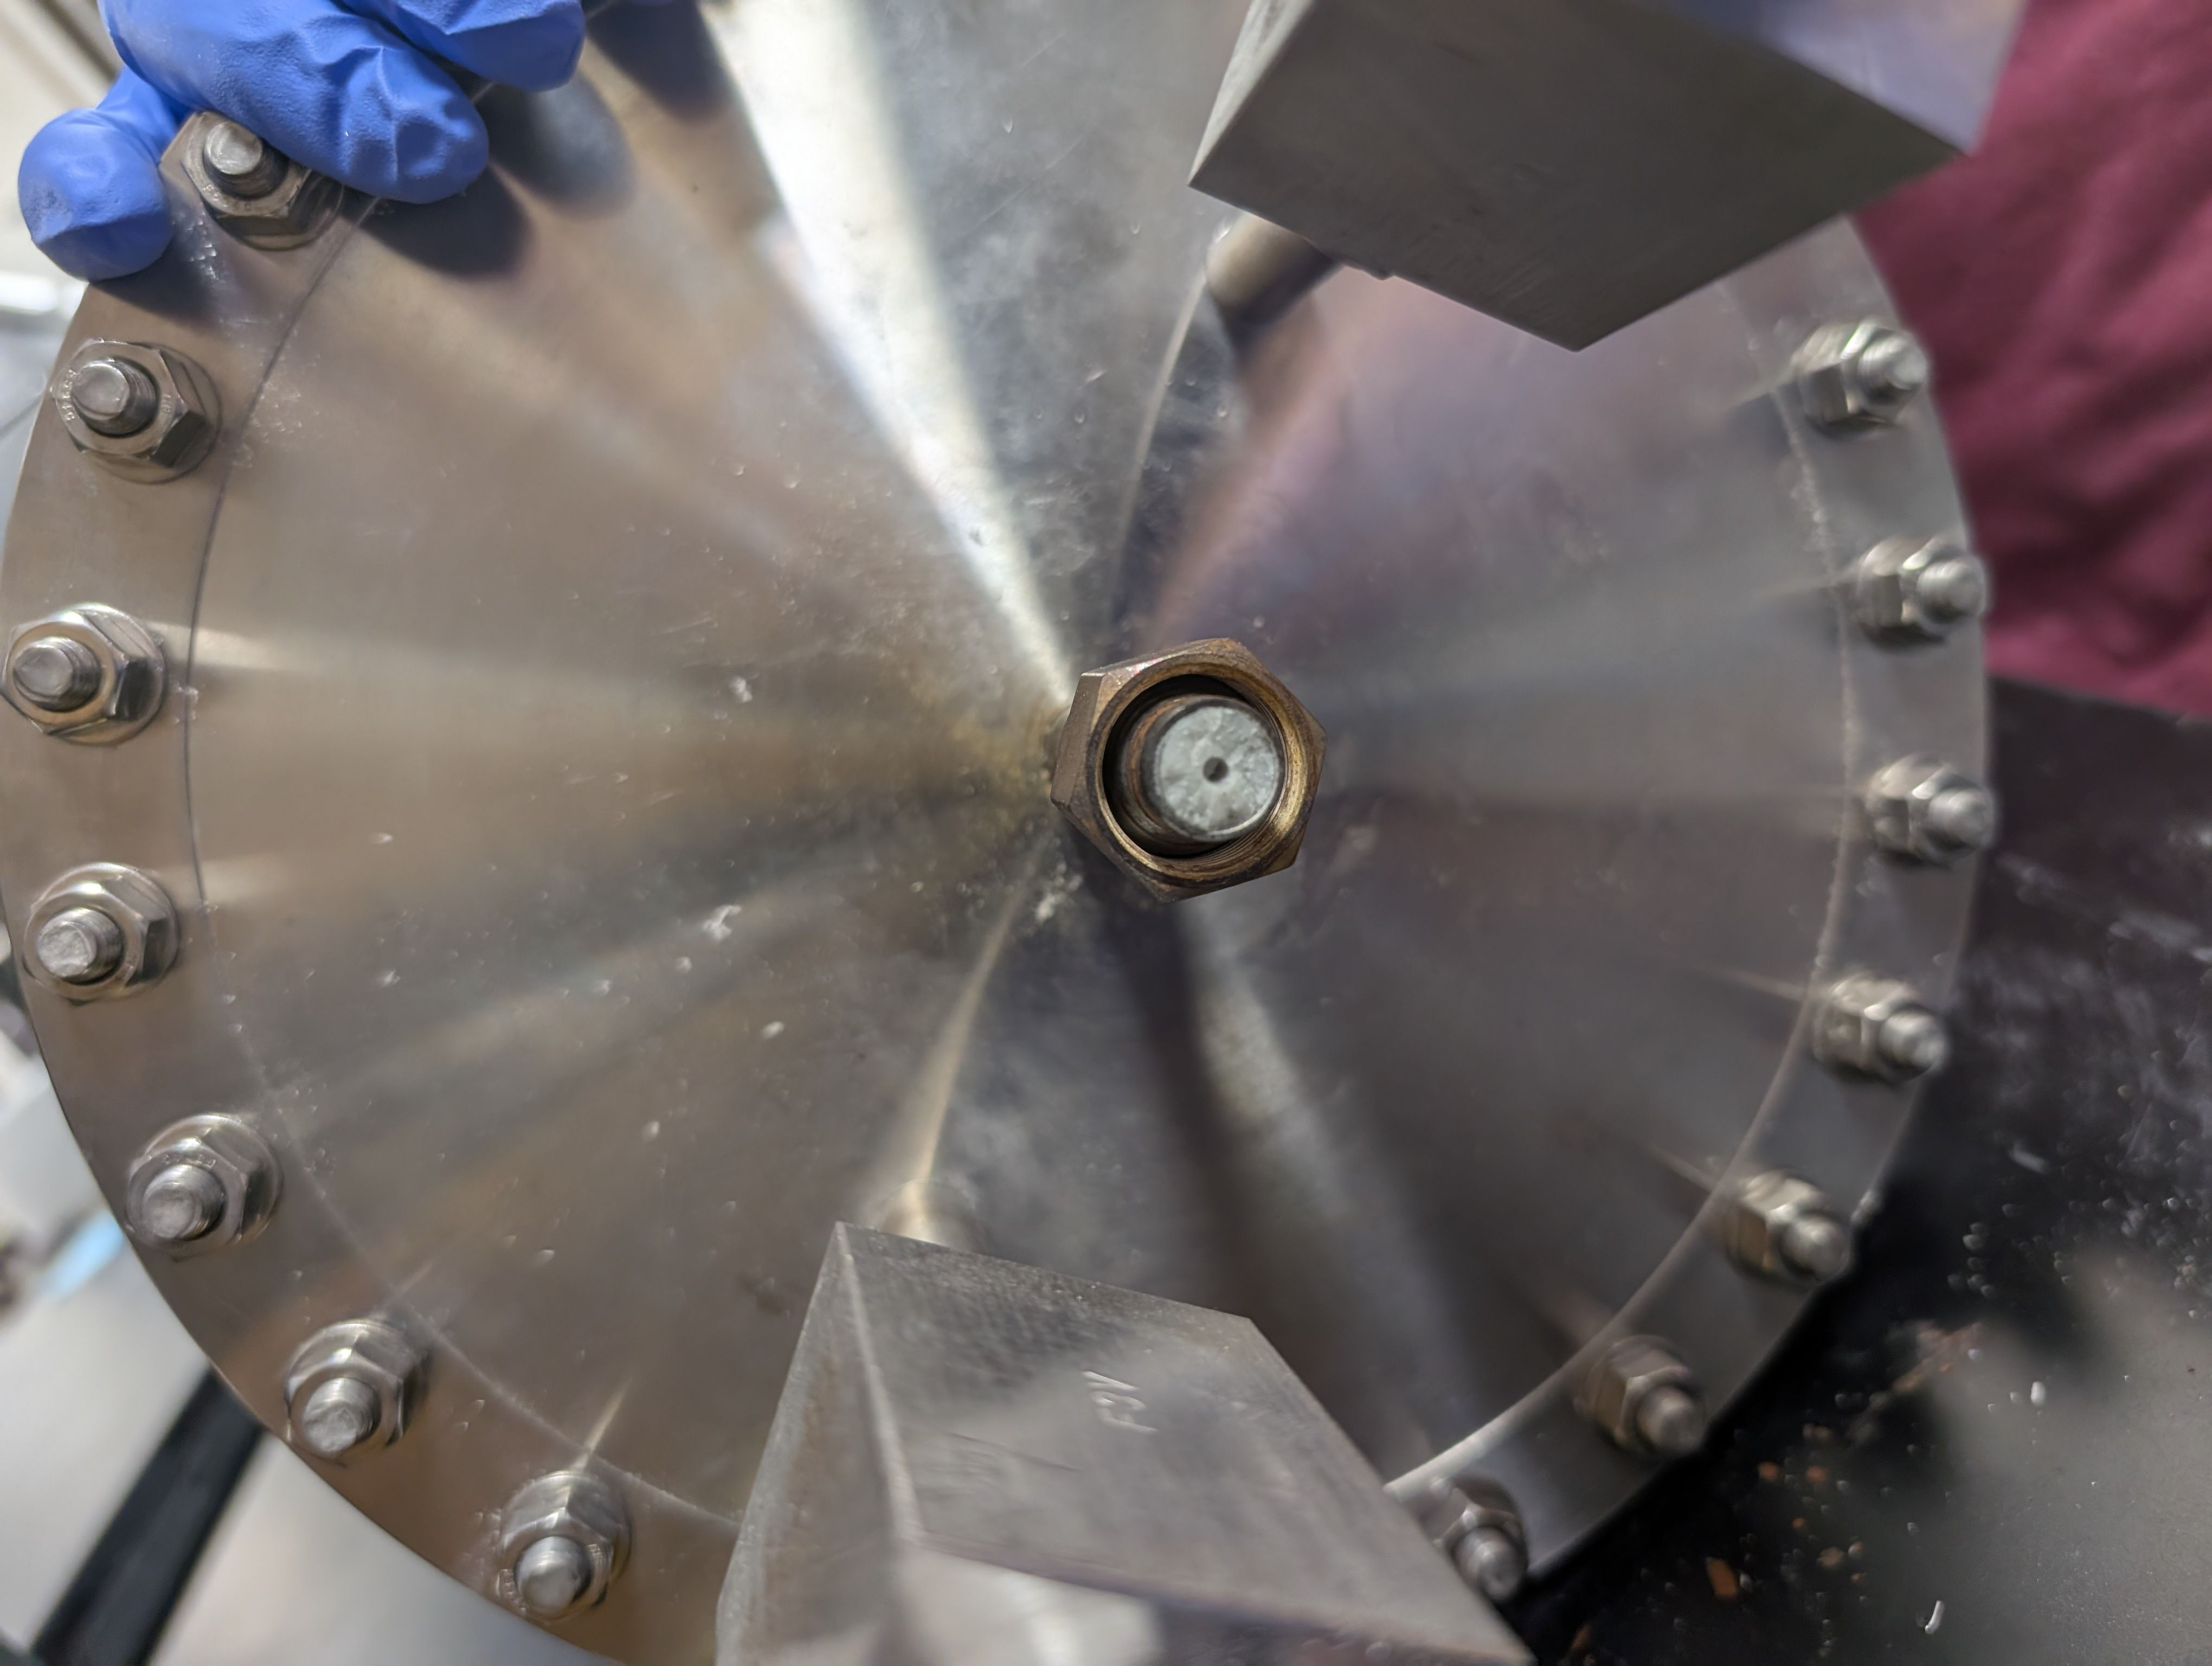
\includegraphics[width=0.6\textwidth]{assets/pictures/transfer lid clog.jpg}
  \caption{Image of salt transfer lid with a salt clog. (3-17-2025)}
  \label{fig: transfer lid clog}
\end{figure}

\begin{figure}[H]
  \centering
  \includegraphics[width=0.6\textwidth]{assets/pictures/needle valve
  clog front.jpg}
  \caption{Image of a clogged Ni needle valve. FLiNaK is visible surrounding the
    center, with a small hole in the center. This shows that FLiNaK
    was freezing at the walls, with only
  a small quantity able to move through the center. (3-17-2025)}
  \label{fig: clogged needle valve front}
\end{figure}

\begin{figure}[H]
  \centering
  \includegraphics[width=0.6\textwidth]{assets/pictures/needle valve
  clog back.jpg}
  \caption{Back of the clogged needle valve. This shows that FLiNaK
    went through the
  valve, but clogged before making its way all the way through. (3-17-2025)}
  \label{fig: clogged needle valve back}
\end{figure}

\begin{figure}[H]
  \centering
  \includegraphics[width=0.6\textwidth]{assets/pictures/total needle valve
  clog.jpg}
  \caption{A fully clogged needle valve, showing that salt slow was
  entirely stopped by this point. (3-17-2025)}
  \label{fig: fully clogged needle valve}
\end{figure}

% TODO: Ask Kyle where he got the large Ni filter.
\begin{figure}
  \centering
  \includegraphics[width=0.6\textwidth]{./assets/pictures/original
  transfer line.jpg}
  \caption{An image of the original transfer line with a large Ni filter on it.
  (9-4-2025)}
  \label{fig: original transfer line}
\end{figure}

% TODO: Find a failure
% \begin{figure}[H]
%   \centering
%   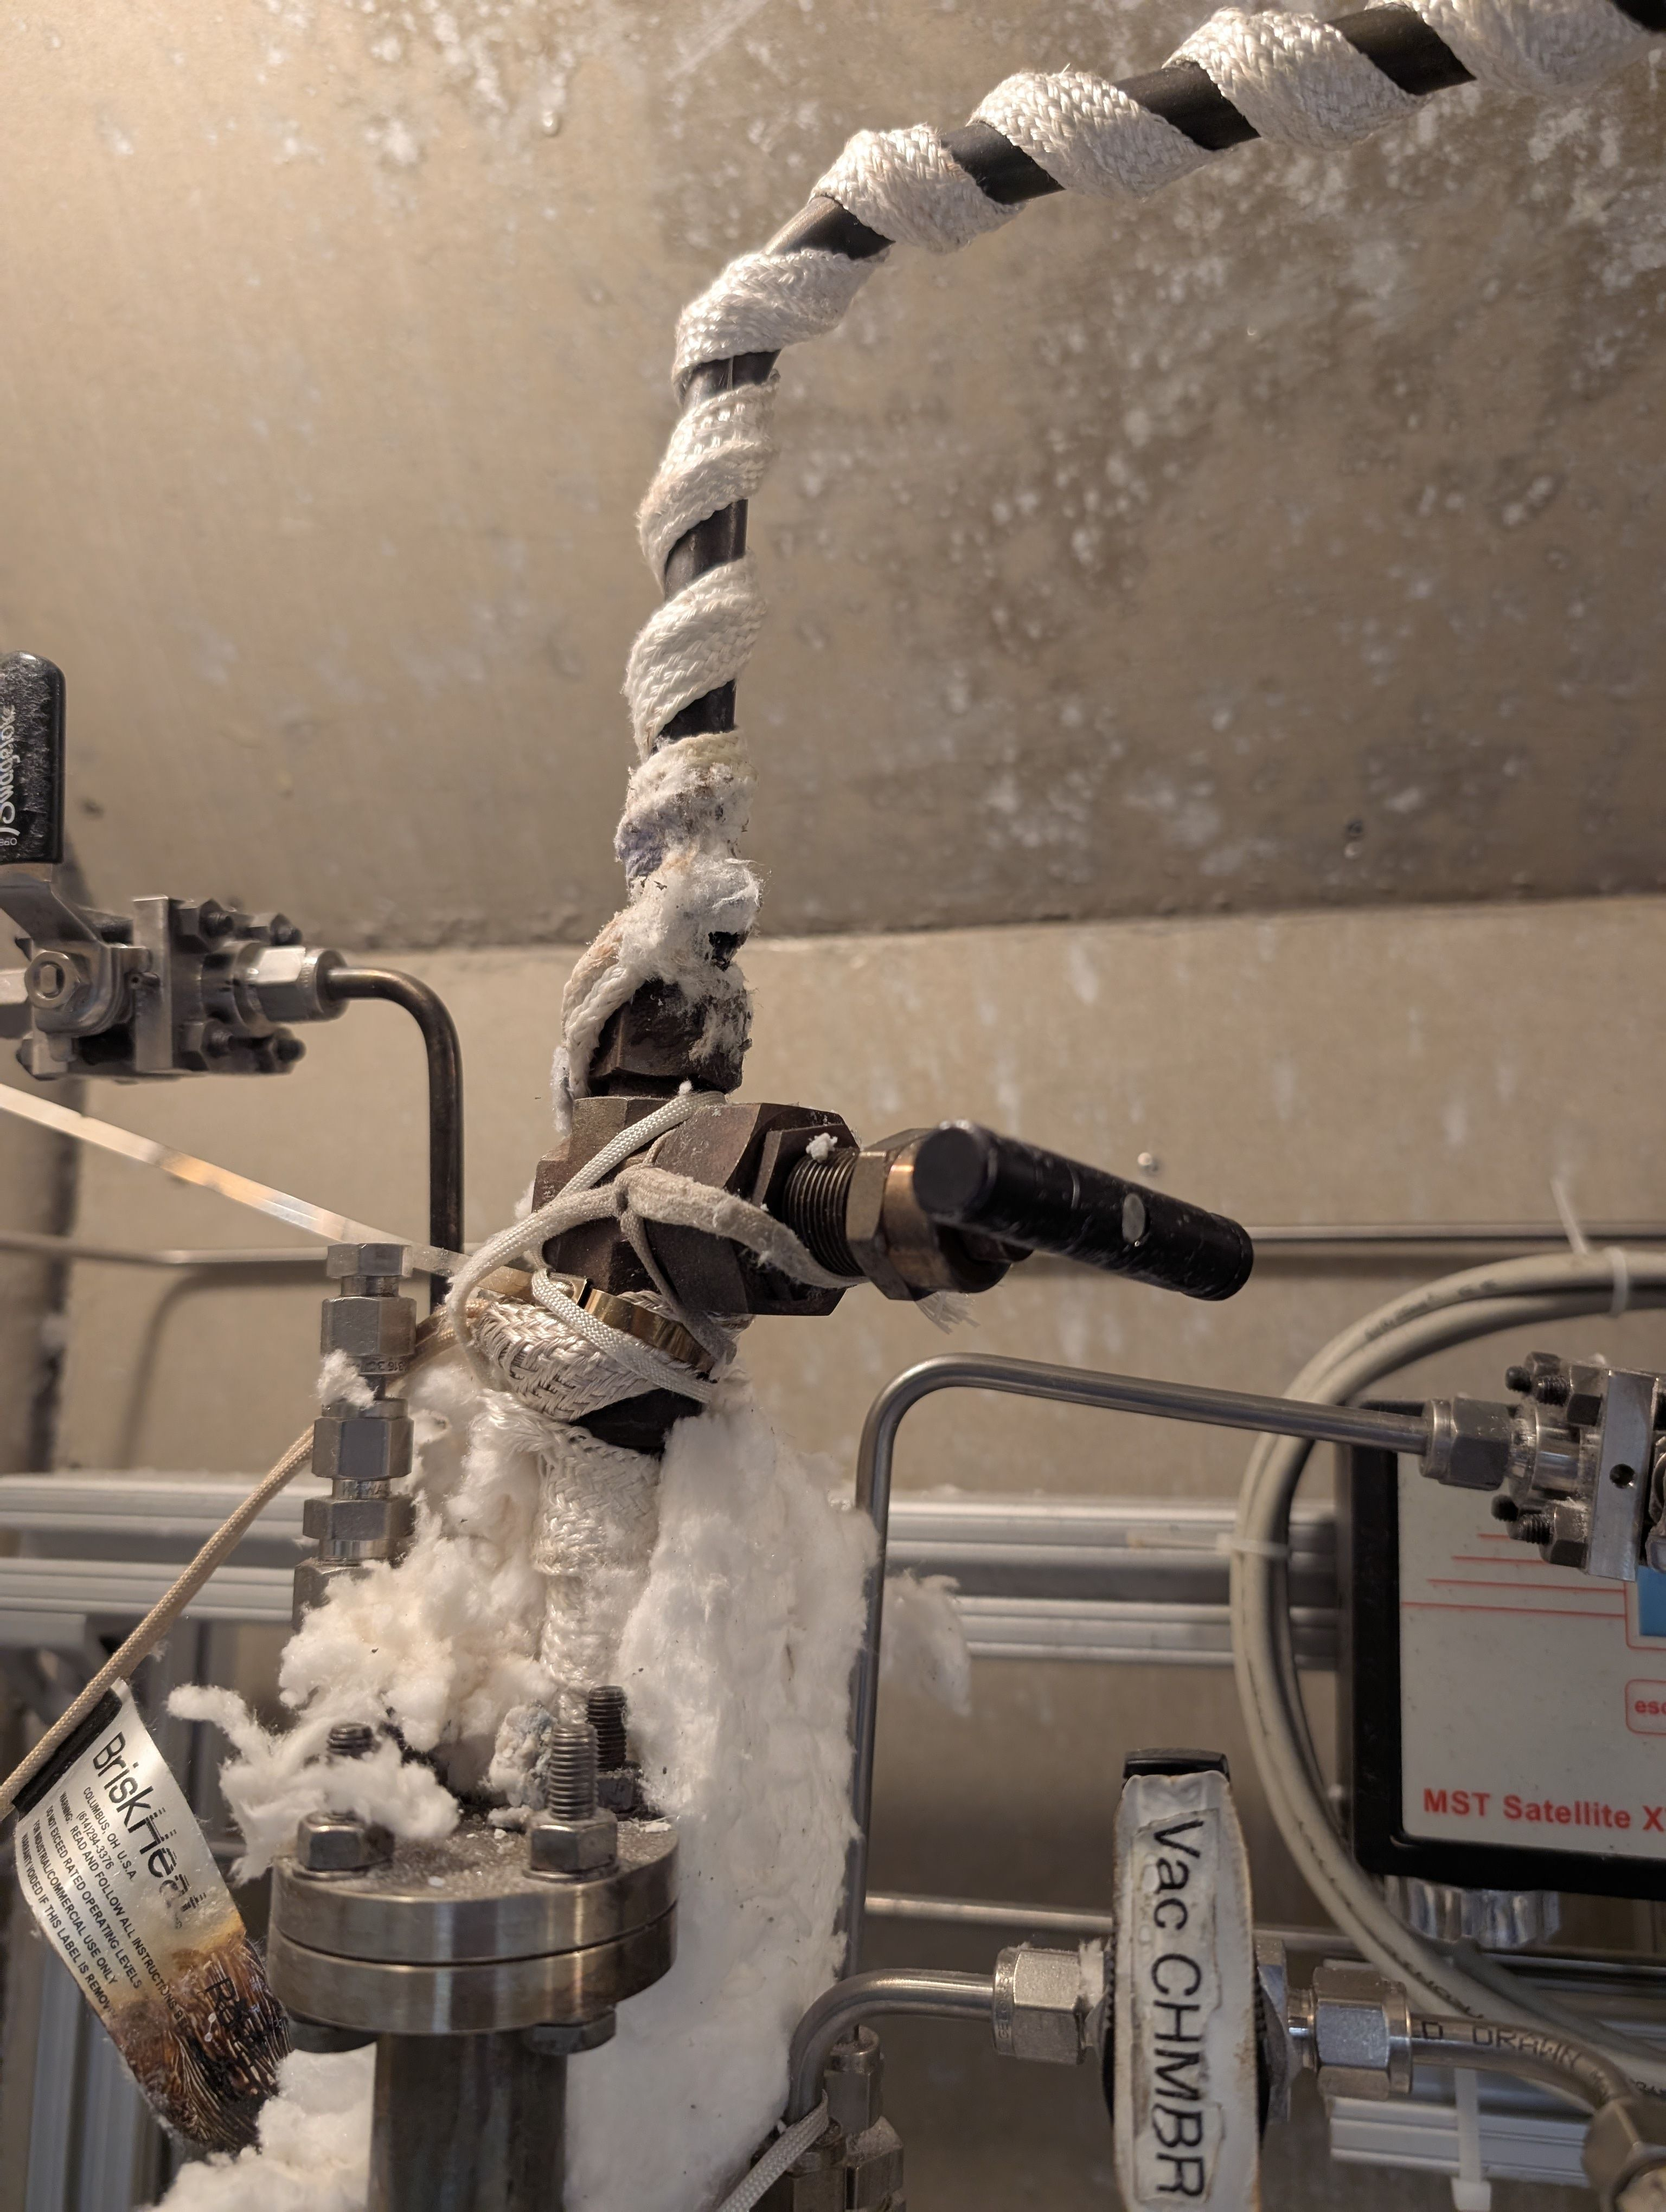
\includegraphics[width=0.6\textwidth]{assets/pictures/heat tape failure.jpg}
%   \caption{A failure in the heat tape. Lack of contact near the
%     needle valve resulted in
%     shorting that caused the heat tape to fail. Note the molten glass near the
%   failure point. (8-18-2025)}
%   \label{fig: heat tape failure}
% \end{figure}

% TODO: Find a picture of the impure FLiNaK that came over following
% purification.
% TODO: If available, get ICPMS data as well.

Following the clog, and failure to melt the salt using a blowtorch,
the transfer line was removed from the system and replaced with a new line. The
original line is shown in \Cref{fig: original transfer line}.
Note that FLiNaK was found throughout the line, indicating full transport of
FLiNaK all the way up to the transfer tank. The tranfer tank also contained a
small quantity of FLiNaK, but it was gray-colored and very impure. There
was a visible clog of FLiNaK coming out of the top of the transfer tank
that had excess FLiNaK coming through. \par

A new transfer line was constructed and placed on the purifier. A smaller
Swagelok micron filter replaced the large Ni filter that was originally
in place. The FLiNaK that was still inside the purifier was repurified,
and a second transfer was attempted. An initial transfer attempt resulted
in a salt freeze. A subsequent attempt to melt the salt in the transfer
line to resume the transfer did not help. This transfer attempt suffered
from heat tape shorting. Due to poor heat transfer, the heat tape used to heat
the line failed and shorted to the metal of the purifier. Blowtorches were
also used to attempt to heat the transfer line, with little success.
The transfer line was then replaced. This second line is shown in
\Cref{fig: second transfer line}.
\par

\begin{figure}
  \centering
  \includegraphics[width=0.6\textwidth]{./assets/pictures/second
  transfer line.jpg}
  \caption{Image of the second transfer line following clogging and removal. It
    is next to the first line, with a brass needle valve in place to prevent the
  FLiNaK inside from escaping. (9-3-2025)}
  \label{fig: second transfer line}
\end{figure}

Following the heat tape failure, changes to the insulation were
made. Originally, Kaowool insulation was placed on the transfer
line with hose clamps made of stainless steel. This was replaced with exhaust
pipe fiberglass tape. The heat tape was then applied on top, and finally
covered with Kaowool. All insulation and heat tape was held in place
using 316L stainless steel zip ties. The transfer tank was also left
with excess heat tape on top
to encourage more heat to be concentrated on the lid of the transfer tank,
discouraging freezing. This worked poorly, and the heat tape
failed and arced. This resulted in molten glass at the arc point.
This was a poor design decision,
as the insulation between the heat tape and the transfer line resulted in the
heat tape heating up excessively, resulting in a failure similar to the
previous attempt, but with more molten glass present. Manual heating with a
blowtorch around the transfer tank lid also resulted in the ball valves on
the transfer tank lid to fail. The seats failed, resulting in loss of vacuum
sealing ability.
\par

Finally, it was determined that tight wrapping, gentle heating, and thorough
temperature monitoring was needed to ensure reliable heating. Five
thermocouples were applied at various points along the transfer line.
One at the base of the transfer line above the reaction chamber.
Heat tape was applied to the transfer line with great care, ensuring there
was no twists or overlap in the tape. Fiberglass tape was then applied on
top, and finally Kaowool was wrapped on the outside of the transfer line.
The on/off heating controller from BriskHeat that was used to control the
temperature of the transfer line was replaced with a Variac. In addition,
three separate heating tapes, each with their own Variac, were used to
implement zone heating. This allowed more power to be applied to some point
of the transfer line compared to others. \par

This same transfer line experienced multiple transfer attempts, each while
salt was present inside the line. During repeated transfer attempts,
the FLiNaK inside the line partially melted and resolidified. When the salt
was melted again, it resulted in expansion and bulging of the transfer line.
This can be seen in \Cref{fig: bulged transfer line}.
On the final transfer attempt, the transfer line was left to slowly heat up
until the FLiNaK inside the line melted. But during this transfer attempt, the
bulged area of the transfer line expanded further, and burst. This resulted in
molten FLiNaK leaking out onto the lid of the reaction chamber. This shorted
the heating tape and resulted in a total system failure, which can
be seen in \Cref{fig: ruptured transfer line} and
\Cref{fig: main failure image}. The subsequent reconstruction and design
improvements are outline in \Cref{sec: reconstruction}. \par

\begin{figure}
  \centering
  \includegraphics[width=0.6\textwidth]{./assets/pictures/bulged
  transfer line.jpg}
  \caption{An image of the bulged transfer line. It is blurred due to poor
  focusing.}
  \label{fig: bulged transfer line}
\end{figure}

\begin{figure}[H]
  \centering
  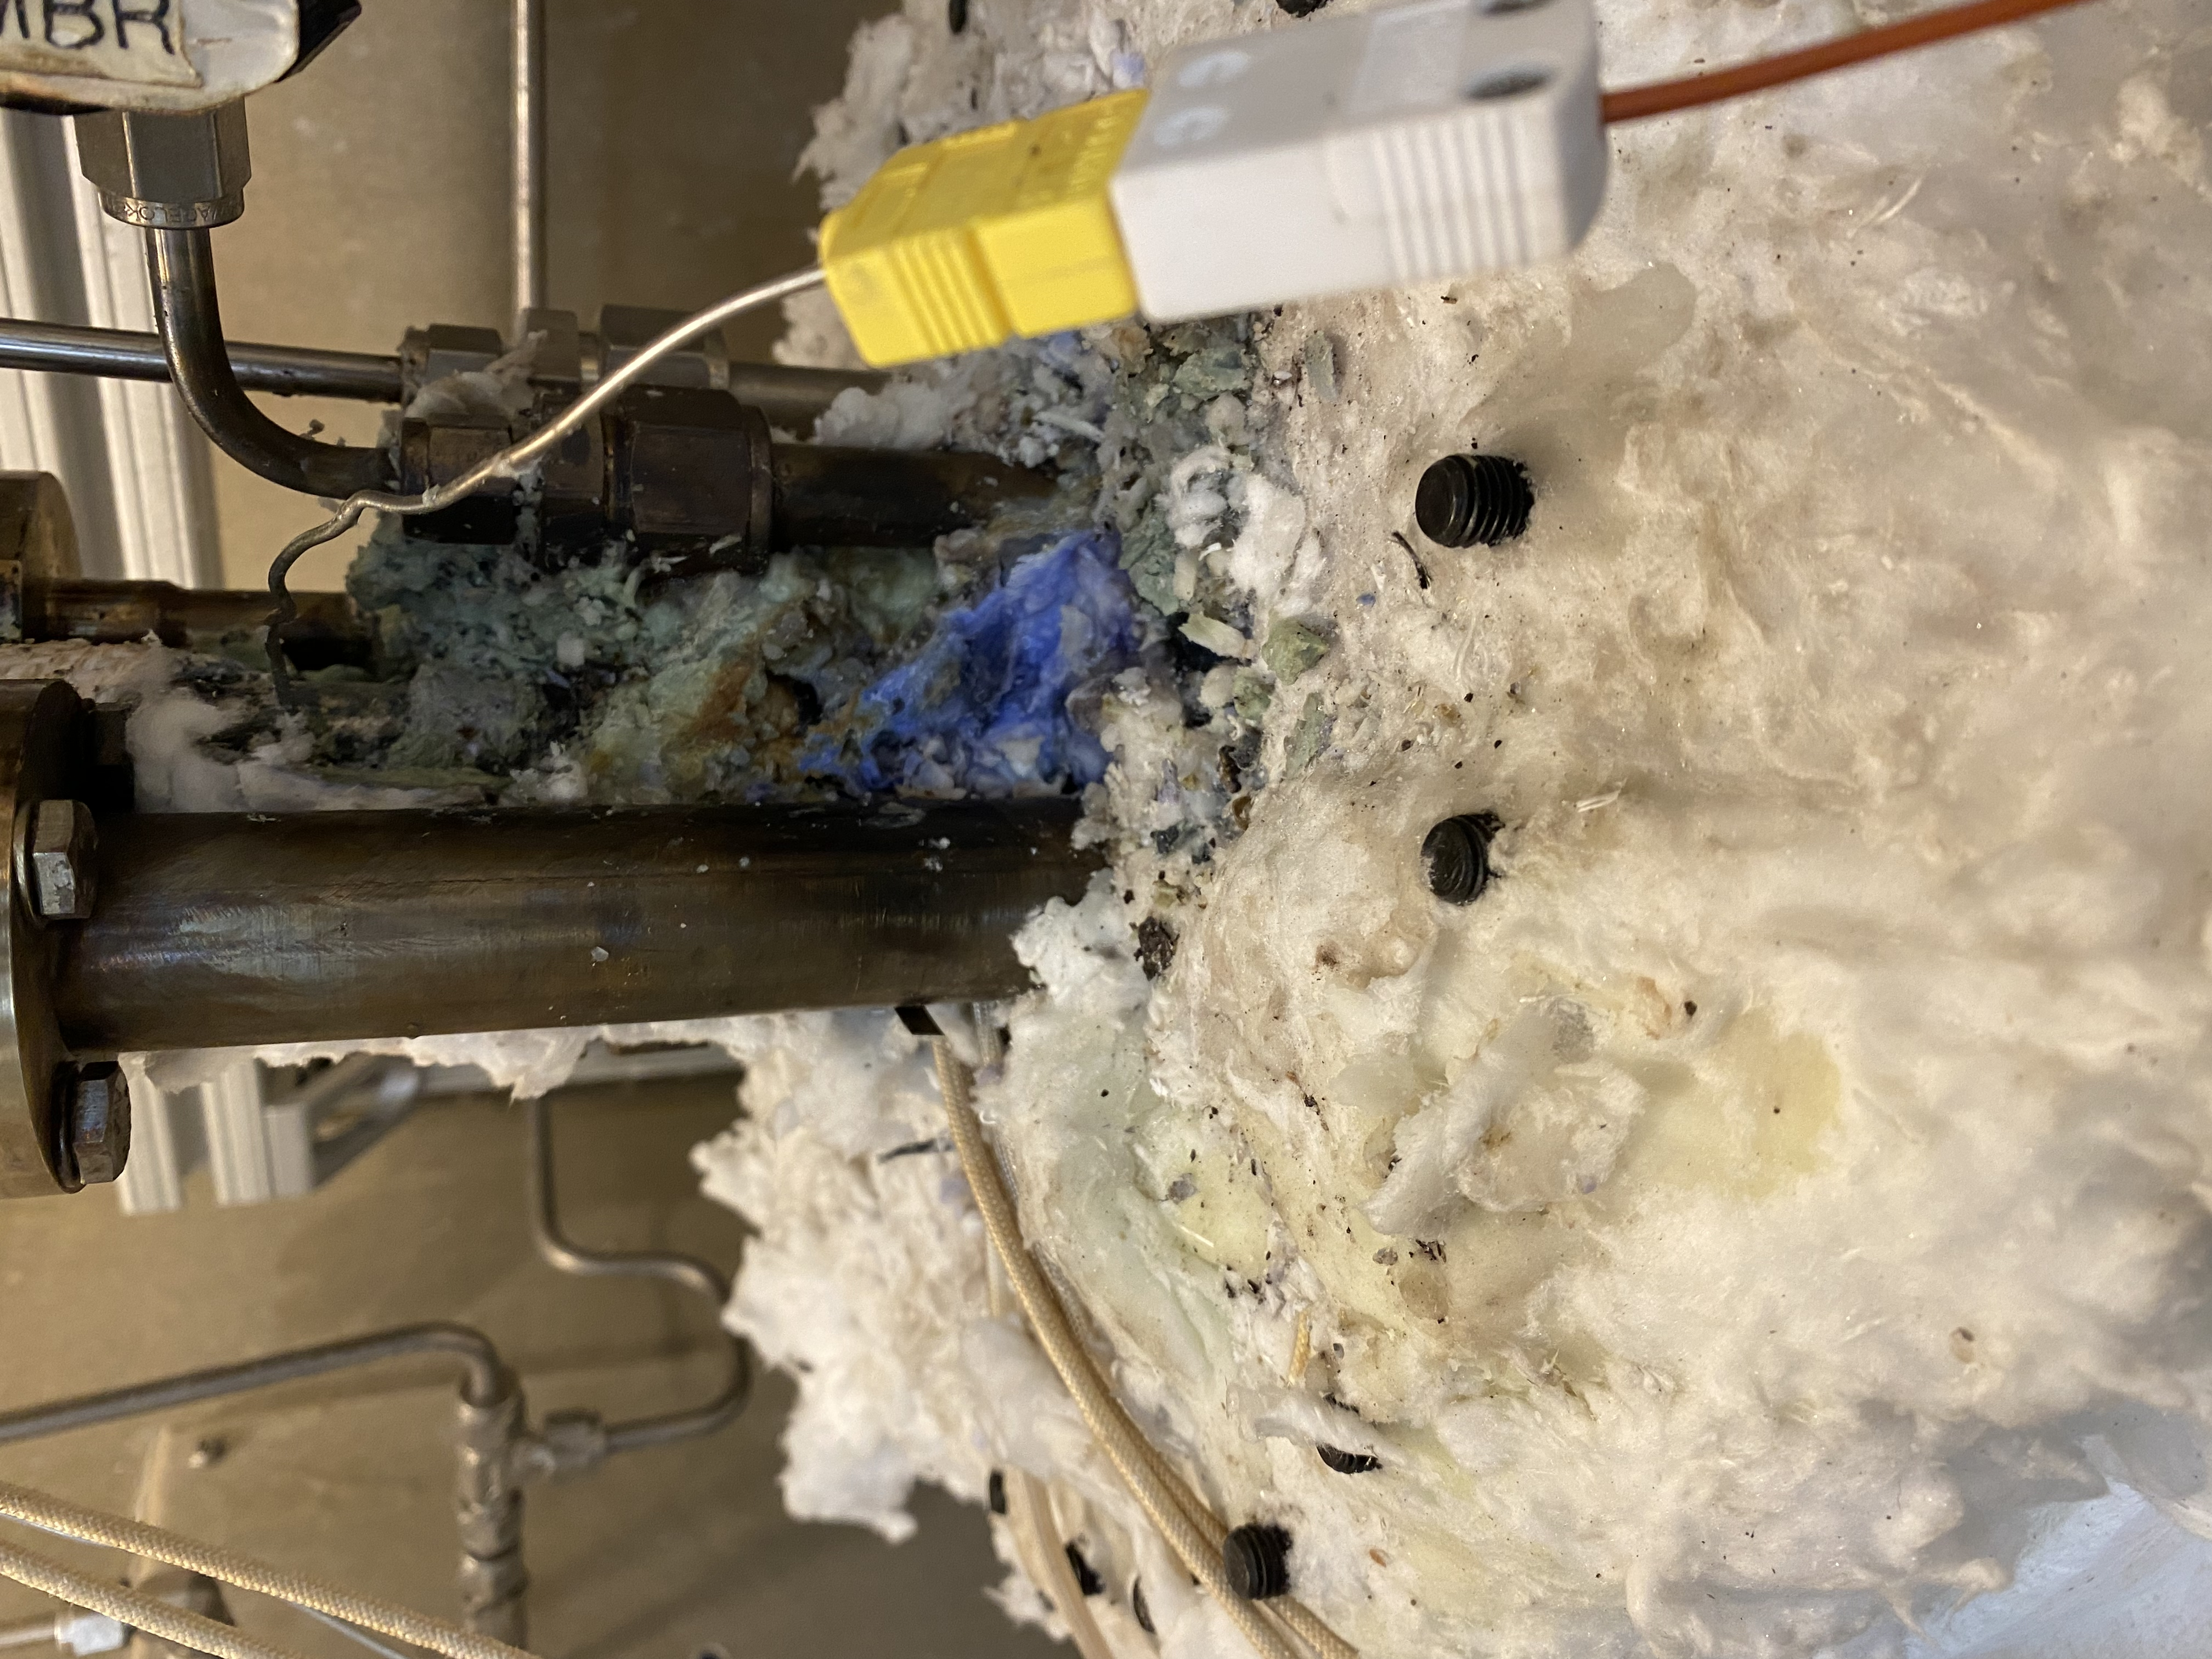
\includegraphics[width=0.6\textwidth,
  angle=270]{./assets/pictures/chamber failure.jpeg}
  \caption{The reaction chamber following the transfer line rupture.
    This was the day after the primary failure. Salt can be seen
    mixed with insulation, and a clear failure is evident. It is yet
  unknown what the blue substance is.  (8-30-2025)}
  \label{fig: ruptured transfer line}
\end{figure}

\begin{figure}
  \centering
  \includegraphics[width=0.6\textwidth]{./assets/pictures/main
  failure image.jpg}
  \caption{An image of the system a few days after the failure with some
    insulation removed. Note the
    molten and discolored alumina insulation, as well as the extensive
  corrosion. (9-2-2024)}
  \label{fig: main failure image}
\end{figure}

Note that the repeated heating/cooling cycles in the presence of FLiNaK
resulted in extensive corrosion of the Ni high temperature needle valves,
as well as the destruction of the stainless steel ferrules used to seal the
fittings connecting the valves to the transfer line. An image of the corroded
ferrule and needle valve is shown in \Cref{fig: corroded needle valve}. There
was also a lack of salt in the transfer line around the reaction chamber,
due to leakage. In \Cref{fig: transfer line inside}, the inside of the
transfer line is devoid of salt, due to leakage. A top-down view inside
the burst area is shown \Cref{fig: reaction chamber line viewkj}.
It should also be noted that all three needle valves used in this system
were completely seized and unable to open or close. This may have partially
been due to corrosion, in addition to the presence of frozen FLiNaK inside
the valve flow path. \par

\begin{figure}
  \centering
  \includegraphics[width=0.6\textwidth]{./assets/pictures/corroded
  needle valve.jpg}
  \caption{An image of the corroded needle valve and ferrule
  following disassembly. (9-4-2025)}
  \label{fig: corroded needle valve}
\end{figure}

\begin{figure}
  \centering
  \includegraphics[width=0.6\textwidth]{./assets/pictures/transfer
  line inside.jpg}
  \caption{The inside of the transfer line following disassembly. Note the
    lack of salt. Having spilled out of the transfer line, there was none
  present in the portion of the line above the reaction chamber. (9-4-2025)}
  \label{fig: transfer line inside}
\end{figure}

\begin{figure}
  \centering
  \includegraphics[width=0.6\textwidth]{./assets/pictures/reaction
  chamber line view.jpg}
  \caption{A top-down view of the top of the reaction chamber
  transfer line (9-4-2025)}
  \label{fig: reaction chamber line view}
\end{figure}

\par

\pagebreak

% \begin{enumerate}% {{{
%   \item The FLiNaK purifier successfully ran twice with hydrogen sparging.
%     The \ch{HF} flow controller was unknowingly not functioning during the
%     runs.
%   \item Following two successful runs, another run was attempted with \ch{HF}
%     running. However, a blowtorch was needed to encourage salt flow
%     during salt transfer.
%   \item The \ch{HF} flow controller was disposed of, and liquid HF
%     buildup inside the
%     feed line was dunked into a \SI{14}{M}
%     % TODO: Confirm 14 M, get original controller model and manufacturer.
%     \ch{KOH} solution.
%   \item An Aalborg controller was used to regulate \ch{HF} flow. The
%     flow was then controlled using LabView. Flow was confirmed by sending
%     \ch{HF} into the bubbler. The buildup of liquid HF was controlled by
%     occasionally closing the HF regulator.
%   \item Purification ran successfully, but the salt clogged in the
%     line when attempting to transfer
%     due to inadequate heating.
%   \item Attempting to transfer, the large Ni filter was clogged,
% and the entire
%     transfer line had to be replaced.
%     % TODO: Confirm the order of events here.
%     % TODO: Include an image of the original filter.
%   \item The in-line filter was replaced with a smaller filter from Swagelok.
%     % TODO: Ask Kyle what the pore size of the SL filter was.
%     % TODO: Include an image of the Swagelok filter
%   \item The purifier was run once again, and the transfer was once
%     again attempted.
%     However, the heating tape used to heat the transfer line was
%     inadequately heated and the tape failed and shorted. This happened during
%     several attempts.
%   \item Exhaust pipe fiber glass insulating wrap was placed around
% the transfer
%     line under the heating
%     tape to attempt to avoid electrical shorting. This worked poorly,
%     as the tape
%     once again failed. Insulating the heat tape resulted in excess
%     heat buildup and
%     failure.
%   \item The tape was again applied directly to the transfer line,
%     followed by fiber glass tape,
%     and finally with Kaowool.
%   \item The tape was carefully wrapped tightly around the transfer
%     line, and a system
%     using 5 thermocouples was used to monitor the temperature of the
%     transfer line.
%   \item This system revealed that the line was not evenly heated, and
%     several points along the
%     transfer line got significantly hotter than other points.
%   \item A Briskheat controller was used previously to control the
%     temperature of the heat tape. This was replaced
%     with a Variac to avoid the overshoot of the on-off behavior of the
%     Briskheat heat tape controllers.
%   \item Multiple heating tapes (controlled with Variacs) were used to
%     attempt zone-heating.
%     This was partially successful, but salt got stuck at the entrance
%     of the transfer tank.
%   \item A large thermal mass of stainless steel at the entrance of
%     the transfer tank (which is 1" thick) caused salt to freeze.
%   \item The final run used a previously frozen transfer line. After a
%     previous run, some bulging was noted on the transfer line near
%     the reaction chamber. However, this was disregarded. In addition,
%     material for a new transfer line was not available, so the existing
%     line was used.
%     \footnote{During these failed attempts, the salt
%       was left inside the reaction chamber, and likely exposed to air
%       throughout. Often, several months went by without any purging or
%       argon cover gas being introduced. As a result, the salt was likely
%     contaminated.}
%   \item While heating the transfer line overnight to attempt to melt
%     the salt contained inside, the transfer line ruptured at the
%     bulging point. This resulted
%     in FLiNaK mixing with the insulation, shorting the heating tape,
%     and ending the
%     attempt. Immediate cleanup was then undertaken by Kyle Williams
%     and Adrian Silva.
%   \item Following the failure, Kyle Williams left Texas A\&M to take
%     a job at Kairos Power. The project was taken over by Nathaniel Thomas.
%   \item Note also that the Ni needle valves would tend to clog with salt, due
%     to the high thermal mass.
%   \item Note that during operation on these attempted transfers, the
%     maximum vacuum that could be pulled on the
%     transfer tank was \SI{4}{Torr}. This indicated the presence of a
%     leak. This may have
%     allowed air into the system, accelerating corrosion, especially
%     at high temperatures.
% \end{enumerate}% }}}

\hrule
\begin{figure}[H]
  \centering
  \includegraphics[width=0.6\textwidth]{assets/pictures/sonicated
  transfer line.jpg}
  \caption{Image of the salt transfer line with a salt clog, from above
  the transfer tank following sonication. (9-2-2025)}
  \label{fig: sonicated transfer line}
\end{figure}

\begin{figure}[H]
  \centering
  \includegraphics[width=0.6\textwidth]{assets/pictures/tape wrapping
  near reaction chamber.jpg}
  \caption{The wrapping of the heat tape near the reaction chamber.
    To encourage contact,
    fiber glass tape was applied with a 316L stainless steel zip tie to hold
  down the heat tape along with the fiber glass tape. (8-18-2025)}
  \label{fig: tape wrapping near reaction chamber}
\end{figure}

\begin{figure}[H]
  \centering
  \includegraphics[width=0.6\textwidth]{assets/pictures/increased
  wrapping density.jpg}
  \caption{Image of increased heat tape wrapping density (less
    spacing between wraps) to encourage
    greater heat transfer. This aims to minimize cold spots in the
    valve that causes clogs. Also note the thermocoulpe placed to
  measure the temperature of the valve. (8-18-2025)}
  \label{fig: increased wrapping density}
\end{figure}

\begin{figure}[H]
  \centering
  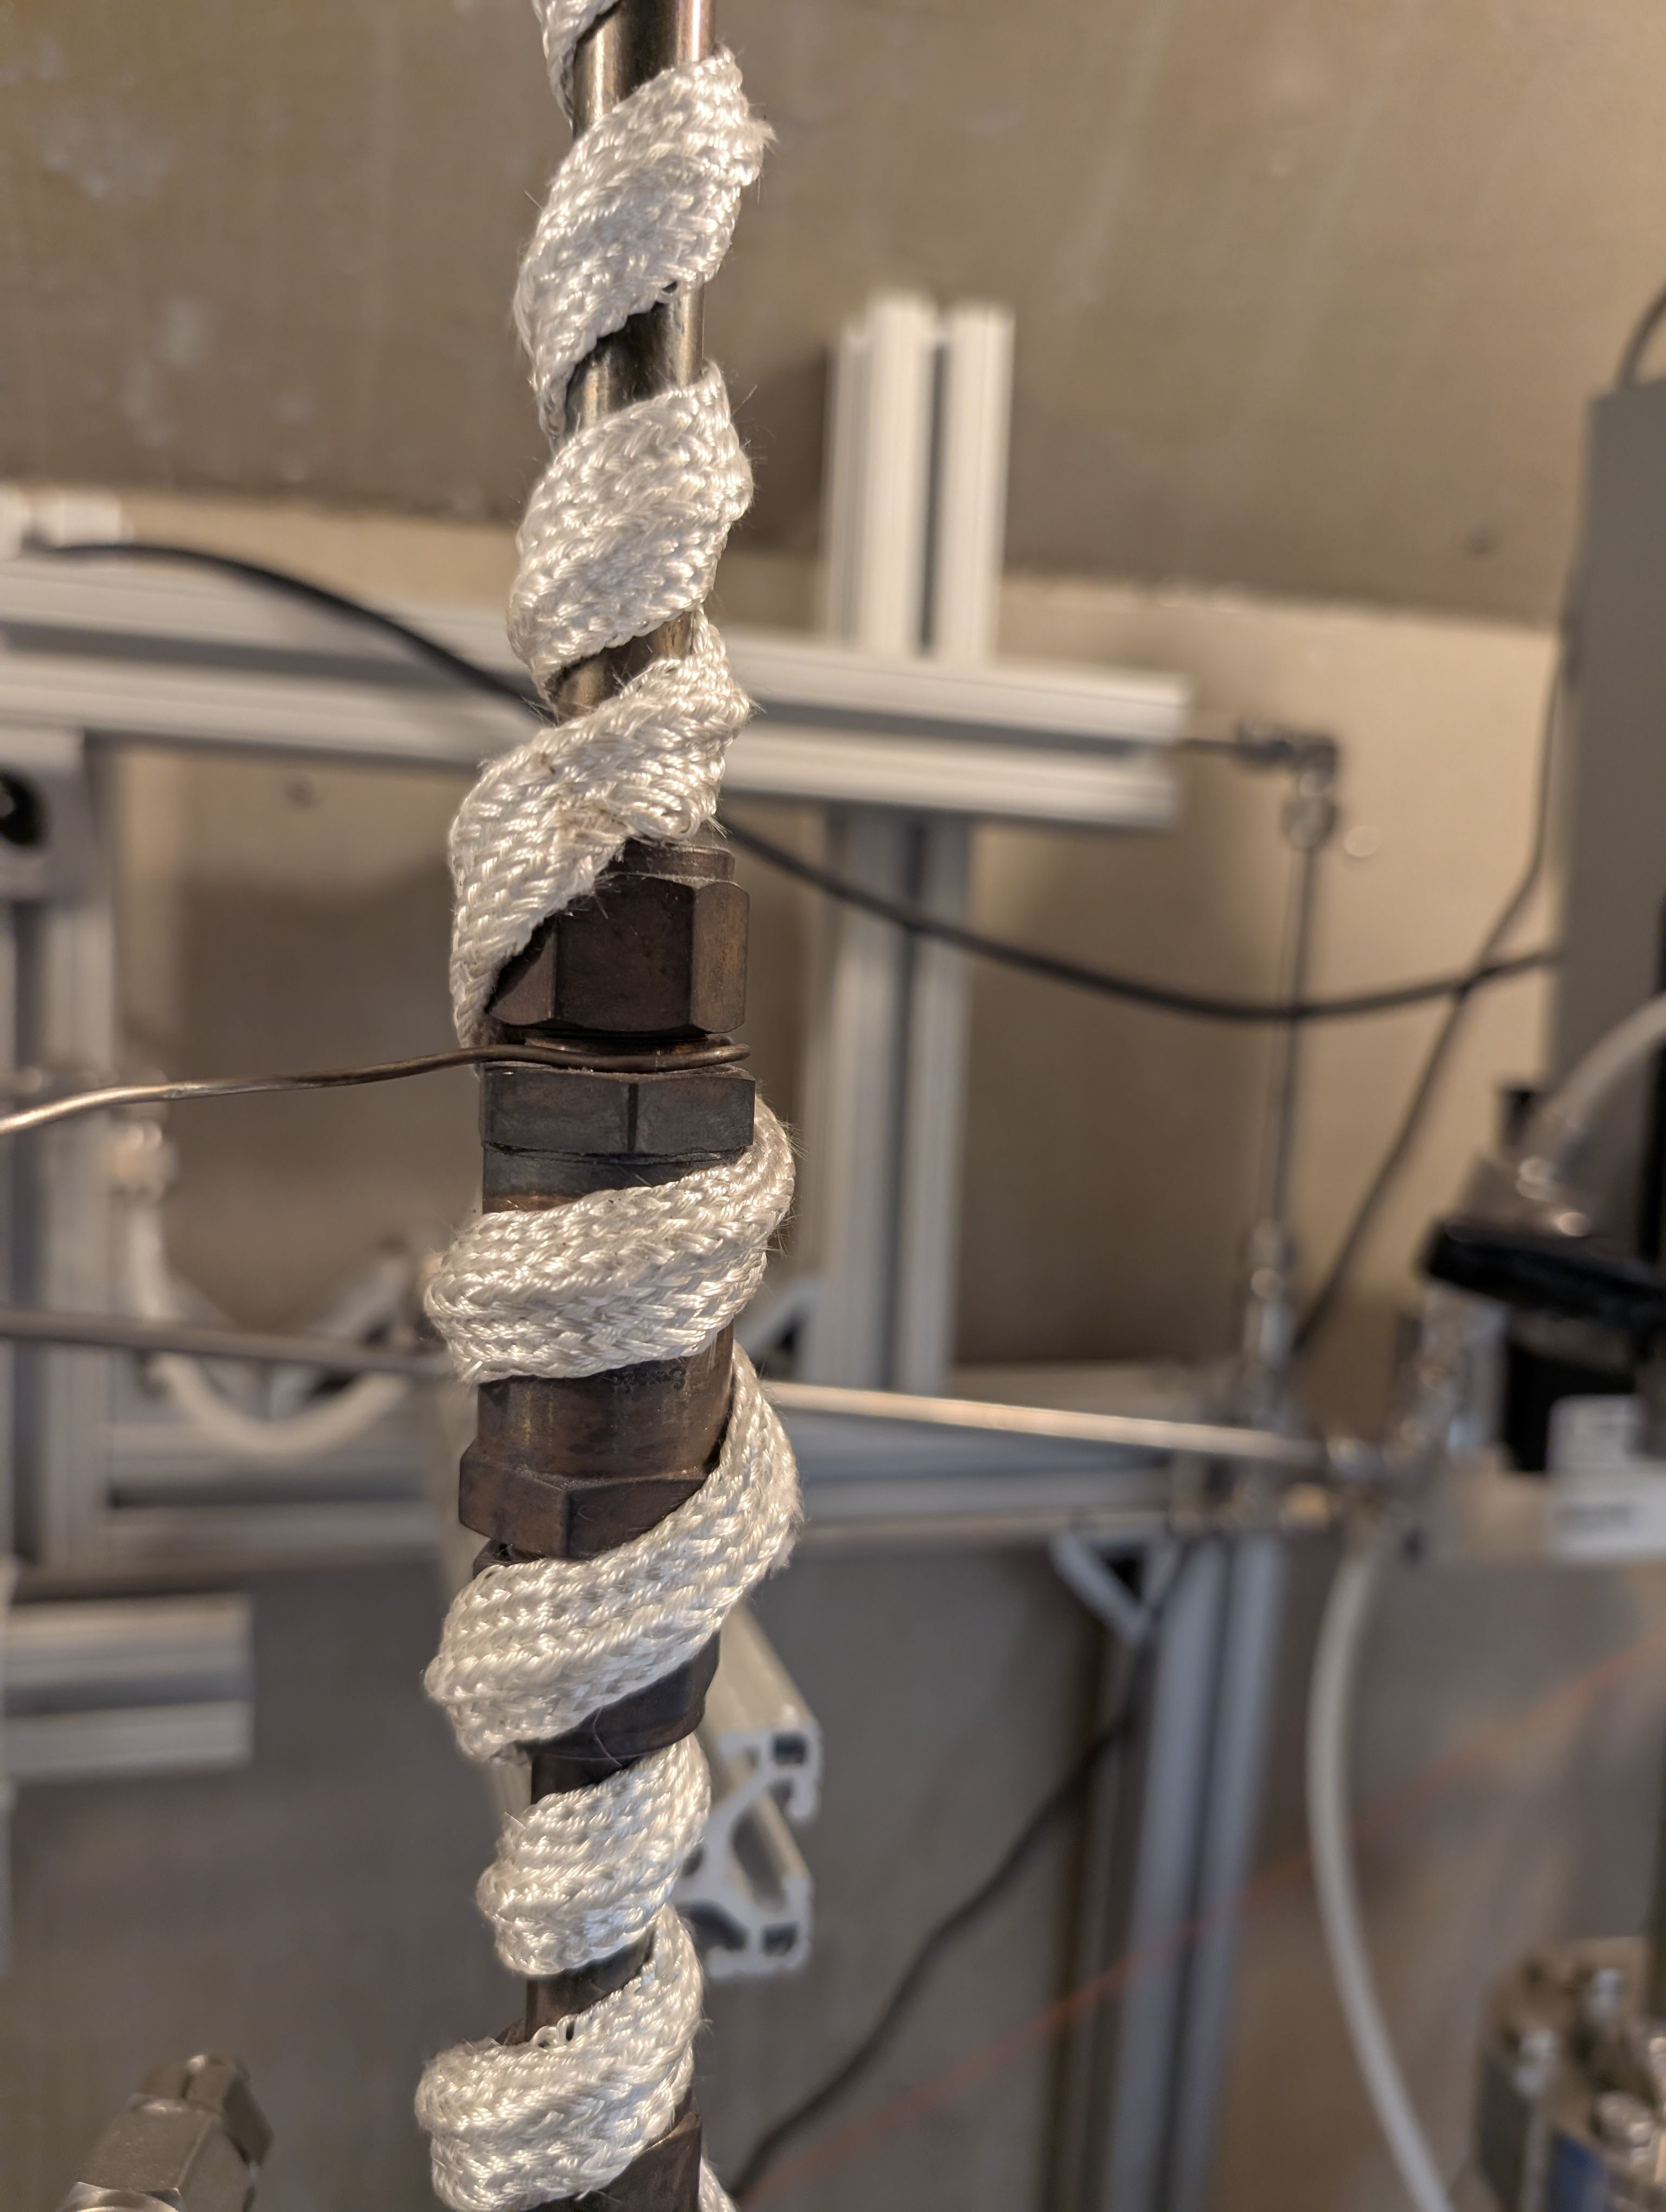
\includegraphics[width=0.6\textwidth]{assets/pictures/filter wrap.jpg}
  \caption{Heating tape wrapped around the in-line salt filter. Note
    the thermocouple
    used to measure the filter temperature. This is another potential
  clog point. (8-18-2025)}
  \label{fig: filter wrap}
\end{figure}

\begin{figure}[H]
  \centering
  \includegraphics[width=0.6\textwidth]{assets/pictures/transfer tank
  valve wrap.jpg}
  \caption{Wrapping of heat tape at the needle valves near the
    transfer tank. Note thermocouples measuring the temperature of both
  valves. (8-18-2025)}
  \label{fig: transfer tank valve wrap}
\end{figure}

\begin{figure}[H]
  \centering
  \includegraphics[width=0.6\textwidth]{assets/pictures/transfer tank
  lid wrap.jpg}
  \caption{Transfer tank lid. Note the excess heat tape and
    thermocouple. The excess tape was used to attempt to heat the
  area near the salt entry point to minize freezing potential. (8-18-2025)}
  \label{fig: transfer tank lid wrap}
\end{figure}

\begin{figure}[H]
  \centering
  \includegraphics[width=0.6\textwidth]{assets/pictures/fully wrapped
  system.jpg}
  \caption{Fully insulated system with Kaowool and fiber glass tape
  to trap heat from heat tape. Note the three needle valves. (8-18-2025)}
  \label{fig: fully wrapped system}
\end{figure}

\begin{figure}[H]
  \centering
  \includegraphics[width=0.6\textwidth]{assets/pictures/ni liner with
  flinak.jpg}
  \caption{The Ni liner with solidified FLiNaK in the bottom. Note
    the severe corrosion. The green color is likely
    \ch{NiF2}. The liquid at the bottom is water that was attracted
    and condensed by the highly hydroscopic FLiNaK. There is about
    \SI{2}{kg} of FLiNaK
  in the bottom of the liner, solidified into a single chunk.}
  \label{fig: ni liner with flinak}
\end{figure}

\begin{figure}[H]
  \centering
  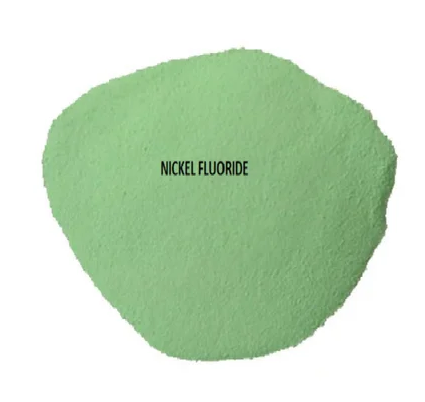
\includegraphics[width=0.6\textwidth]{assets/pictures/ni fluoride.png}
  \caption{\ch{NiF2}. The green color is likely the same green
    substance on the corroded surfaces inside of
    the reaction chamber. Taken from
  \href{https://www.indiamart.com/proddetail/nickel-fluoride-electroplating-grade-2850552649991.html}{indiamart.com}}
  \label{fig: ni fluoride}
\end{figure}

\begin{figure}[H]
  \centering
  \includegraphics[width=0.6\textwidth]{assets/pictures/chamber with
  liner and lid removed.jpg}
  \caption{\ch{NiF2}. The reaction chamber with the liner and the lid removed.
    Note the severely corroded copper gasket, a potential contributor
    to the poor vacuum. The green material around the gasket is
    likely copper (ii) fluoride dihydrate, a turquoise
  material. (11-11-2025)}
  \label{fig: chamber with liner and lid removed}
\end{figure}

\begin{figure}[H]
  \centering
  \includegraphics[width=0.6\textwidth]{assets/pictures/corroded
  copper gasket.jpg}
  \caption{The corroded copper gasket of the reaction chamber. (11-11-2025)}
  \label{fig: corroded copper gasket}
\end{figure}

\begin{figure}[H]
  \centering
  \includegraphics[width=0.6\textwidth]{assets/pictures/copper
  fluoride dihydrate.jpg}
  \caption{Copper fluoride dihydrate, the substance that likely
    formed around the copper gasket of the reaction chamber. Taken from
  \href{https://chemcraft.su/product/24304}{chemcraft.su}.}
  \label{fig: copper fluoride dihydrate}
\end{figure}

\begin{figure}[H]
  \centering
  \includegraphics[width=0.6\textwidth]{assets/pictures/dirty
  reaction chamber with no gasket.jpg}
  \caption{Dirty reaction chamber with no gasket. Note that the
  knife-edge of the CF flange appears to be intact. (11-11-2025)}
  \label{fig: dirty reaction chamber with no gasket}
\end{figure}

\begin{figure}[H]
  \centering
  \includegraphics[width=0.6\textwidth]{assets/pictures/molten flinak
  in old liner.png}
  \caption{Molten FLiNaK in the old liner. Note the solid material on
    the liquid surface. Likely
    oxides with high melting temperature. The liner was placed inside
    of the furnace to melt the
    salt, allowing the dip tubes to be freed. It took about 4 hours
    at \SI{700}{\celsius} to melt the
    salt and pull the dip tubes free. The HF inside the fume hood
    reached about \SI{2}{ppm} before the
    lid was removed, and around \SI{20}{ppm} after it was removed.
    Full PPE, including nitrile + fiber glass
    high temperature mitts were used, as well as a full face
    respirator with new HF filters. The room was also cleared
  while the operation was conducted. (11-12-2025)}
  \label{fig: molten flinak in old liner}
\end{figure}

\begin{figure}[H]
  \centering
  \includegraphics[width=0.6\textwidth]{assets/pictures/liner with
  flinak better lighting.jpg}
  \caption{The old Ni liner with better lighting. The salt at the
    bottom is visibly green. Clearly
  very contaminated, likely with Ni fluoride. (11-25-2026)}
  \label{fig: liner with flinak better lighting}
\end{figure}

\begin{figure}[H]
  \centering
  \includegraphics[width=0.6\textwidth]{assets/pictures/dip tubes
  after being pulled.jpg}
  \caption{The reaction chamber dip tubes after being removed from
  the molten FLiNaK. Note the extensive corrosion. (11-25-2026)}
  \label{fig: dip tubes after being pulled}
\end{figure}

\begin{figure}[H]
  \centering
  \includegraphics[width=0.6\textwidth]{./assets/pictures/reaction
  chamber lid after being pulled.jpg}
  \caption{The reaction chamber lid after being pulled from the
  molten FLiNaK. (11-25-2026)}
  \label{fig: reaction chamber lid after being pulled}
\end{figure}

\begin{figure}[H]
  \centering
  \includegraphics[width=0.6\textwidth]{./assets/pictures/bottom of
  reaction chamber after pull.jpg}
  \caption{The reaction chamber bottom after being pulled. Note the
    extensive corrosion and liquid at the
    bottom. Likely, some FLiNaK either leaked out, or vaporized and
    redeposited on the bottom of the chamber.
    Water is accumulated from exposure to atmosphere. The clean
    copper gasket is a
  new, unexposed gasket placed to protect the knife edge. (11-25-2026)}
  \label{fig: bottom of reaction chamber after pull}
\end{figure}

\begin{figure}[H]
  \centering
  \includegraphics[width=0.6\textwidth]{./assets/pictures/gas tube
  upper portion.jpg}
  \caption{The gas bubbler dip tube removed from the reaction
    chamber. Note the two breaches in the stem region. This likely
    resulted in improper gas flow/bubbling through the salt. The
    tube was cut into multiple portions in the effort to remove it from
    the reaction chamber lid. Hammering resulted in the tube bending as
  well. (01-16-2026)}
  \label{fig: gas tube upper portion}
\end{figure}

\begin{figure}[H]
  \centering
  \includegraphics[width=0.6\textwidth]{./assets/pictures/gas tube
  lower portion.jpg}
  \caption{The lower portion of the gas bubbler dip tube (01-16-2026)}
  \label{fig: gas tube lower portion}
\end{figure}

\begin{figure}[H]
  \centering
  \includegraphics[width=0.6\textwidth]{./assets/pictures/gas tube
  upper portion rupture.jpg}
  \caption{A close-up of the rupture in the upper portion of the gas
  dip tube. (01-16-2026)}
  \label{fig: gas tube upper portion rupture}
\end{figure}

\begin{figure}[H]
  \centering
  \includegraphics[width=0.6\textwidth]{./assets/pictures/lid after
  gas tube removal.jpg}
  \caption{The reaction chamber lid after the gas tube was removed.
    The thermocouple well was
    also removed. The remaining tube is the salt transfer tube, partially cut
  in an effort to remove it from the reaction chamber lid. (01-16-2026)}
  \label{fig: lid after gas tube removal}
\end{figure}

\begin{figure}[H]
  \centering
  \includegraphics[width=0.6\textwidth]{./assets/pictures/salt
  transfer line cut closeup.jpg}
  \caption{The salt transfer line cut to remove it from the transfer
  lid (close-up). (01-16-2026)}
  \label{fig: salt transfer line cut closeup}
\end{figure}

\begin{figure}[H]
  \centering
  \includegraphics[width=0.6\textwidth]{./assets/pictures/transfer
  line clog during removal.jpg}
  \caption{A FLiNaK clog found in the salt transfer line during disassembly.
    Even after washing, some salt remained. A half-face respirator with HF
    filters was worn during this disassembly, and a shop vac was used
    to clean any residual powders generated
    from cutting and hammering. All FLiNaK residue was placed into a
    solid waste bag, and tools exposed to FLiNaK were cleaned with
  tap water. (01-16-2026)}
  \label{fig: transfer line clog during removal}
\end{figure}

\begin{figure}[H]
  \centering
  \includegraphics[width=0.6\textwidth]{./assets/pictures/transfer
  and gas bubbler lines.jpg}
  \caption{The gas bubbler dip tube and salt transfer dip tubes after
  removal. (01-16-2026)}
  \label{fig: transfer and gas bubbler lines}
\end{figure}

\begin{figure}[H]
  \centering
  \includegraphics[width=0.6\textwidth]{./assets/pictures/salt dip
  tube partial rupture.jpg}
  \caption{Close up of the salt transfer line partial rupture.
    Possibly caused by a combination of thermal stress
  and corrosion. (01-16-2026)}
  \label{fig:salt dip tube partial rupture}
\end{figure}

\begin{figure}[H]
  \centering
  \includegraphics[width=0.6\textwidth]{./assets/pictures/salt dip
  tube upper portion.jpg}
  \caption{Close up of the middle-upper portion of the salt transfer
  line. No apparent damage. (01-16-2026)}
  \label{fig:salt dip tube upper portion}
\end{figure}

\begin{figure}[H]
  \centering
  \includegraphics[width=0.6\textwidth]{./assets/pictures/salt
  transfer reducer.jpg}
  \caption{Close up of the reducer used to couple the transfer line
    to the lid. This part was coated with molten FLiNaK during the line
  rupture. (01-16-2026)}
  \label{fig:salt transfer reducer}
\end{figure}

\begin{figure}[H]
  \centering
  \includegraphics[width=0.6\textwidth]{./assets/pictures/transfer
  line bulge back.jpg}
  \caption{Back of the ruptured portion of the salt transfer line.
    Bulging is visible, induced by thermal
  expansion of salt when melting. (01-16-2026)}
  \label{fig:transfer line bulge back}
\end{figure}

\begin{figure}[H]
  \centering
  \includegraphics[width=0.6\textwidth]{./assets/pictures/salt
  transfer top-down inside view.jpg}
  \caption{Top-down view of the transfer line, showing narrowing and
  corrosion inside the line. (01-16-2026)}
  \label{fig:salt transfer top-down inside view}
\end{figure}

\begin{figure}[H]
  \centering
  \includegraphics[width=0.6\textwidth]{./assets/pictures/transfer
  line total clog inside.jpg}
  \caption{A cut-away view of the upper portion of the transfer line,
  showing a clog. (01-16-2026)}
  \label{fig:transfer line total clog inside}
\end{figure}

\begin{figure}[H]
  \centering
  \includegraphics[width=0.6\textwidth]{./assets/pictures/reaction
  chamber lid bottom no tubes.jpg}
  \caption{A cut-away view of the upper portion of the transfer line,
  showing a clog. (01-16-2026)}
  \label{fig:reaction chamber lid bottom no tubes}
\end{figure}

\begin{figure}[H]
  \centering
  \includegraphics[width=0.6\textwidth]{./assets/pictures/top of
  reaction chamber lid with tubes removed.jpg}
  \caption{Reaction chamber lid top with all tubes removed. (01-16-2026)}
  \label{fig:top of reaction chamber lid with tubes removed}
\end{figure}

\begin{figure}[H]
  \centering
  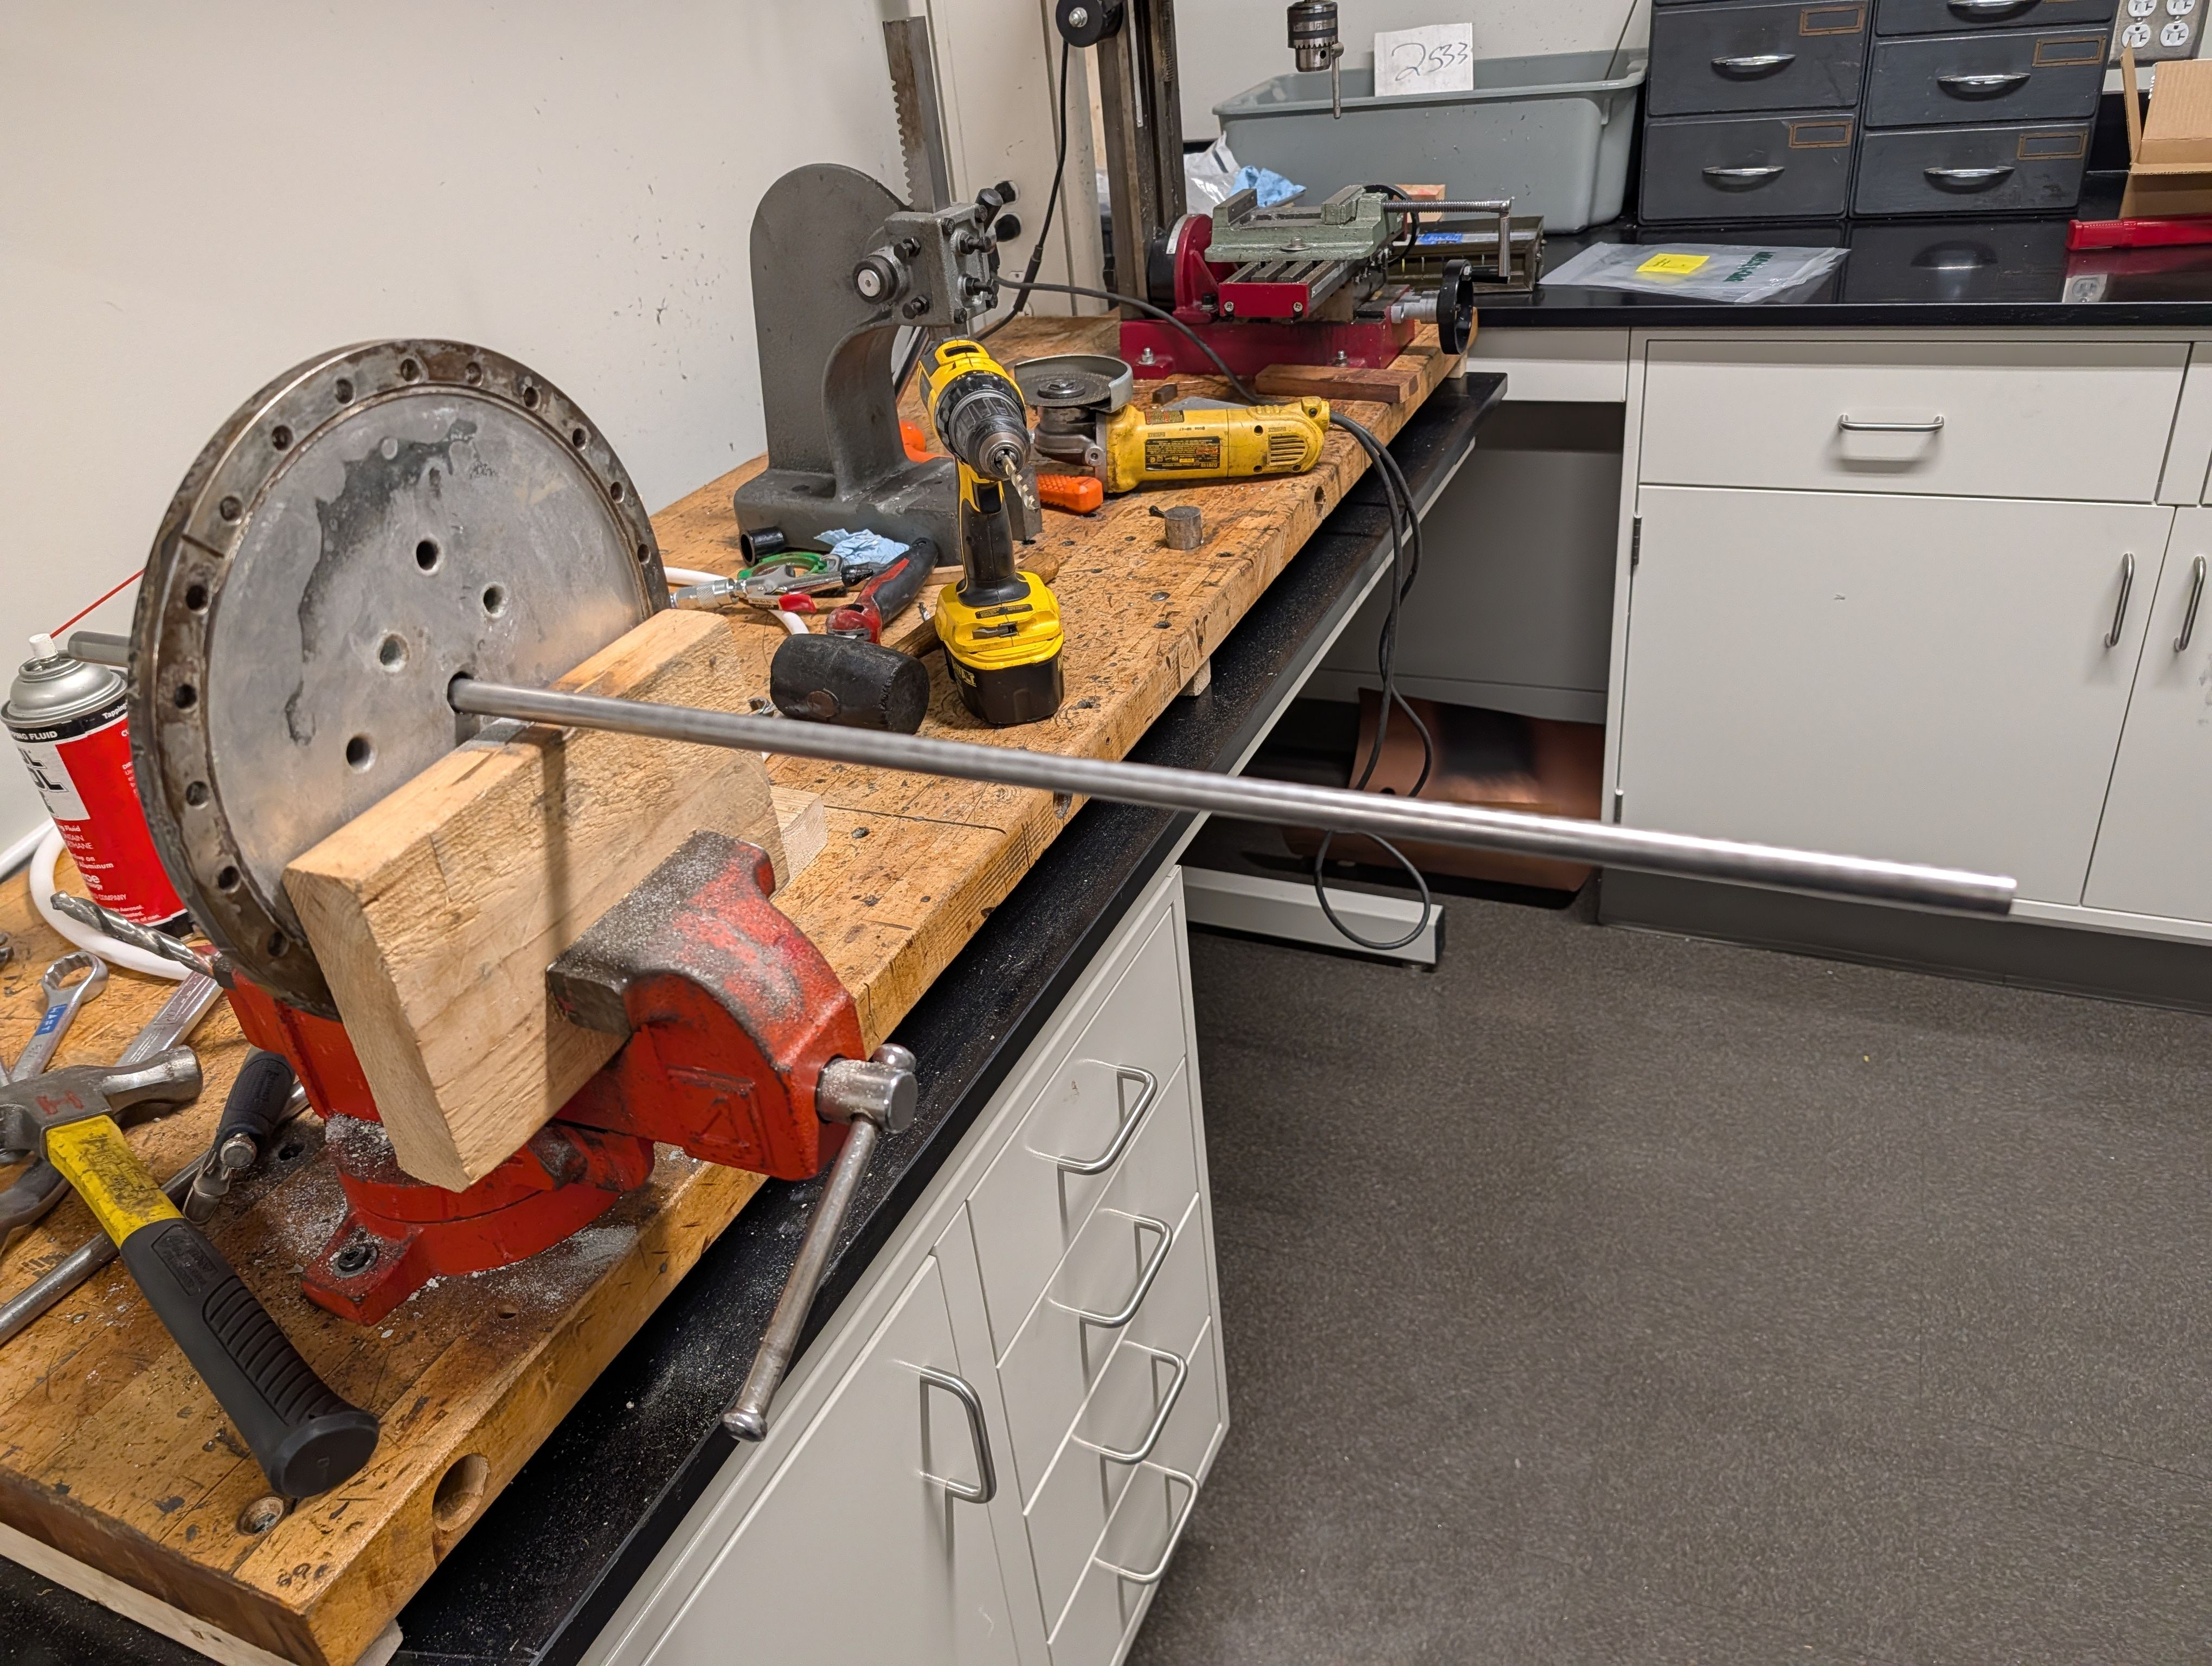
\includegraphics[width=0.6\textwidth]{./assets/pictures/new c276 dip tube.jpg}
  \caption{New C276 salt transfer dip tube shown in the reaction
  chamber lid. (01-16-2026)}
  \label{fig:new c276 dip tube}
\end{figure}

\begin{figure}[H]
  \centering
  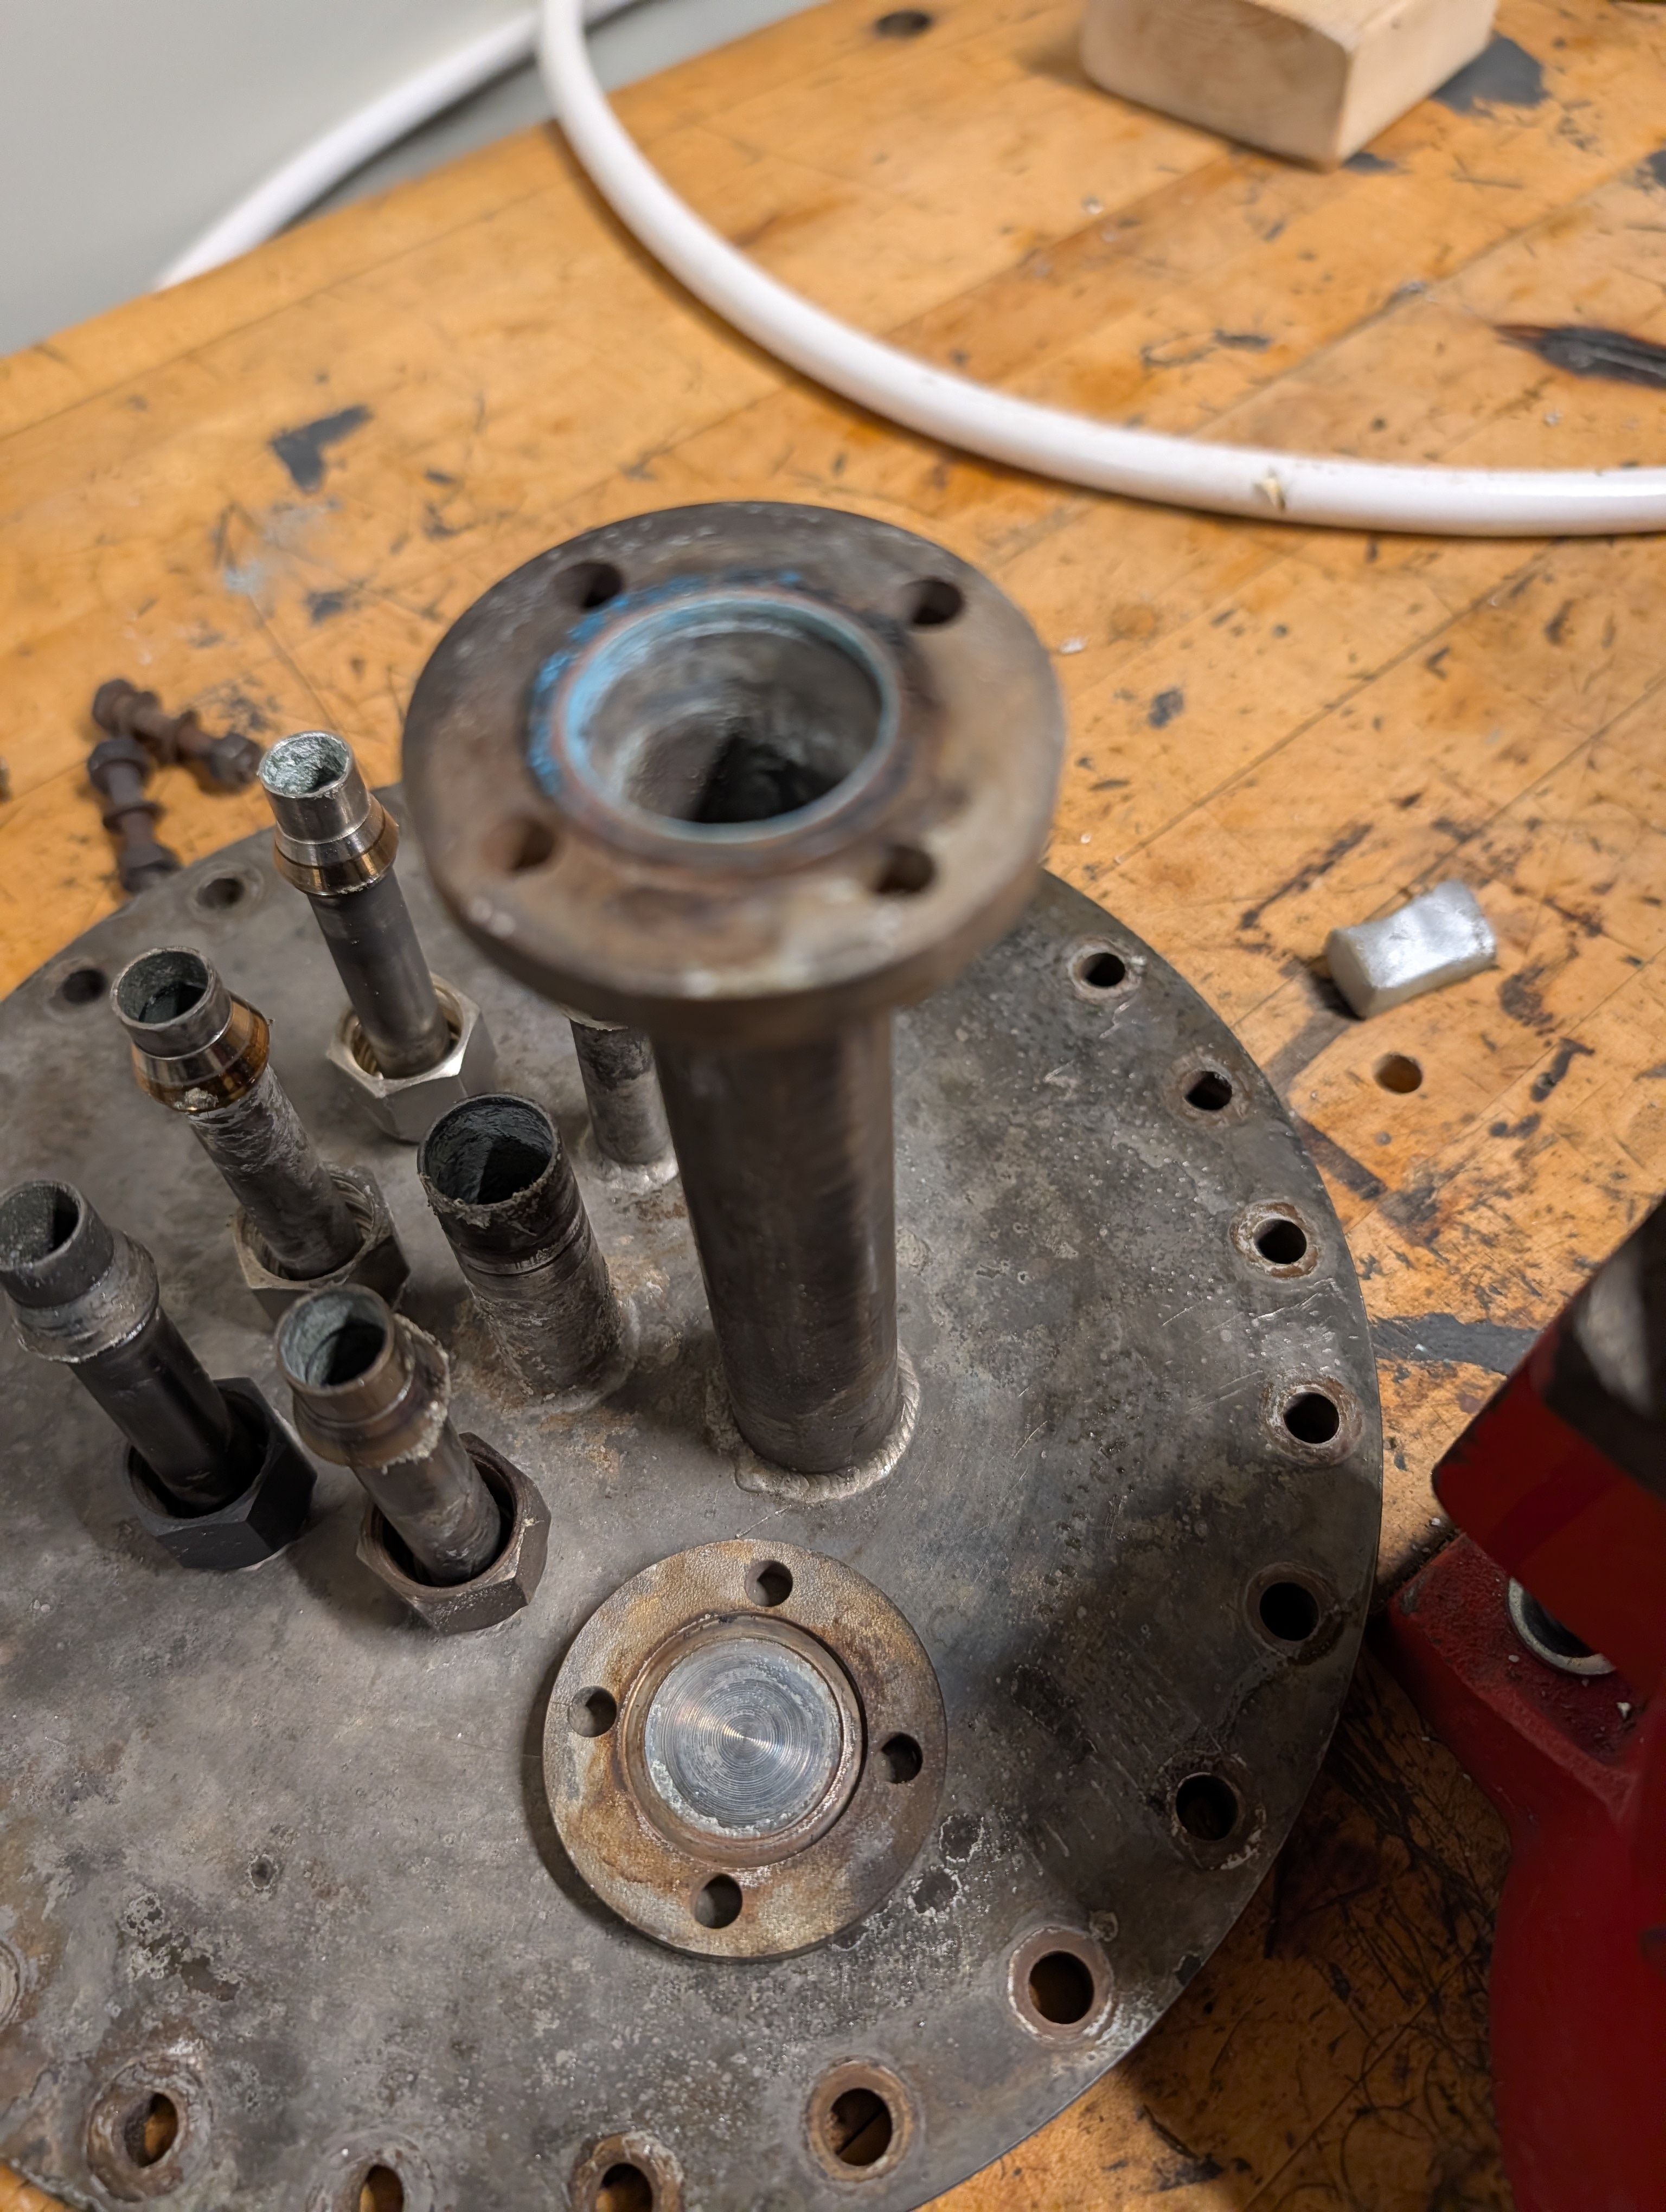
\includegraphics[width=0.6\textwidth]{./assets/pictures/salt feed port.jpg}
  \caption{View of the salt feed port. Note the light corrosion
  around the copper gasket. (01-16-2026)}
  \label{fig:salt feed port}
\end{figure}

\begin{figure}[H]
  \centering
  \includegraphics[width=0.6\textwidth]{./assets/pictures/top down
  view of salt feed port.jpg}
  \caption{Top-down view of the salt feed port. Note the corrosion
    along the inside wall.
    Even though there is no direct contact with salt, the atmosphere
  inside the reaction chamber enabled corrosion.(01-16-2026)}
  \label{fig:top down view of salt feed port}
\end{figure}

\begin{figure}[H]
  \centering
  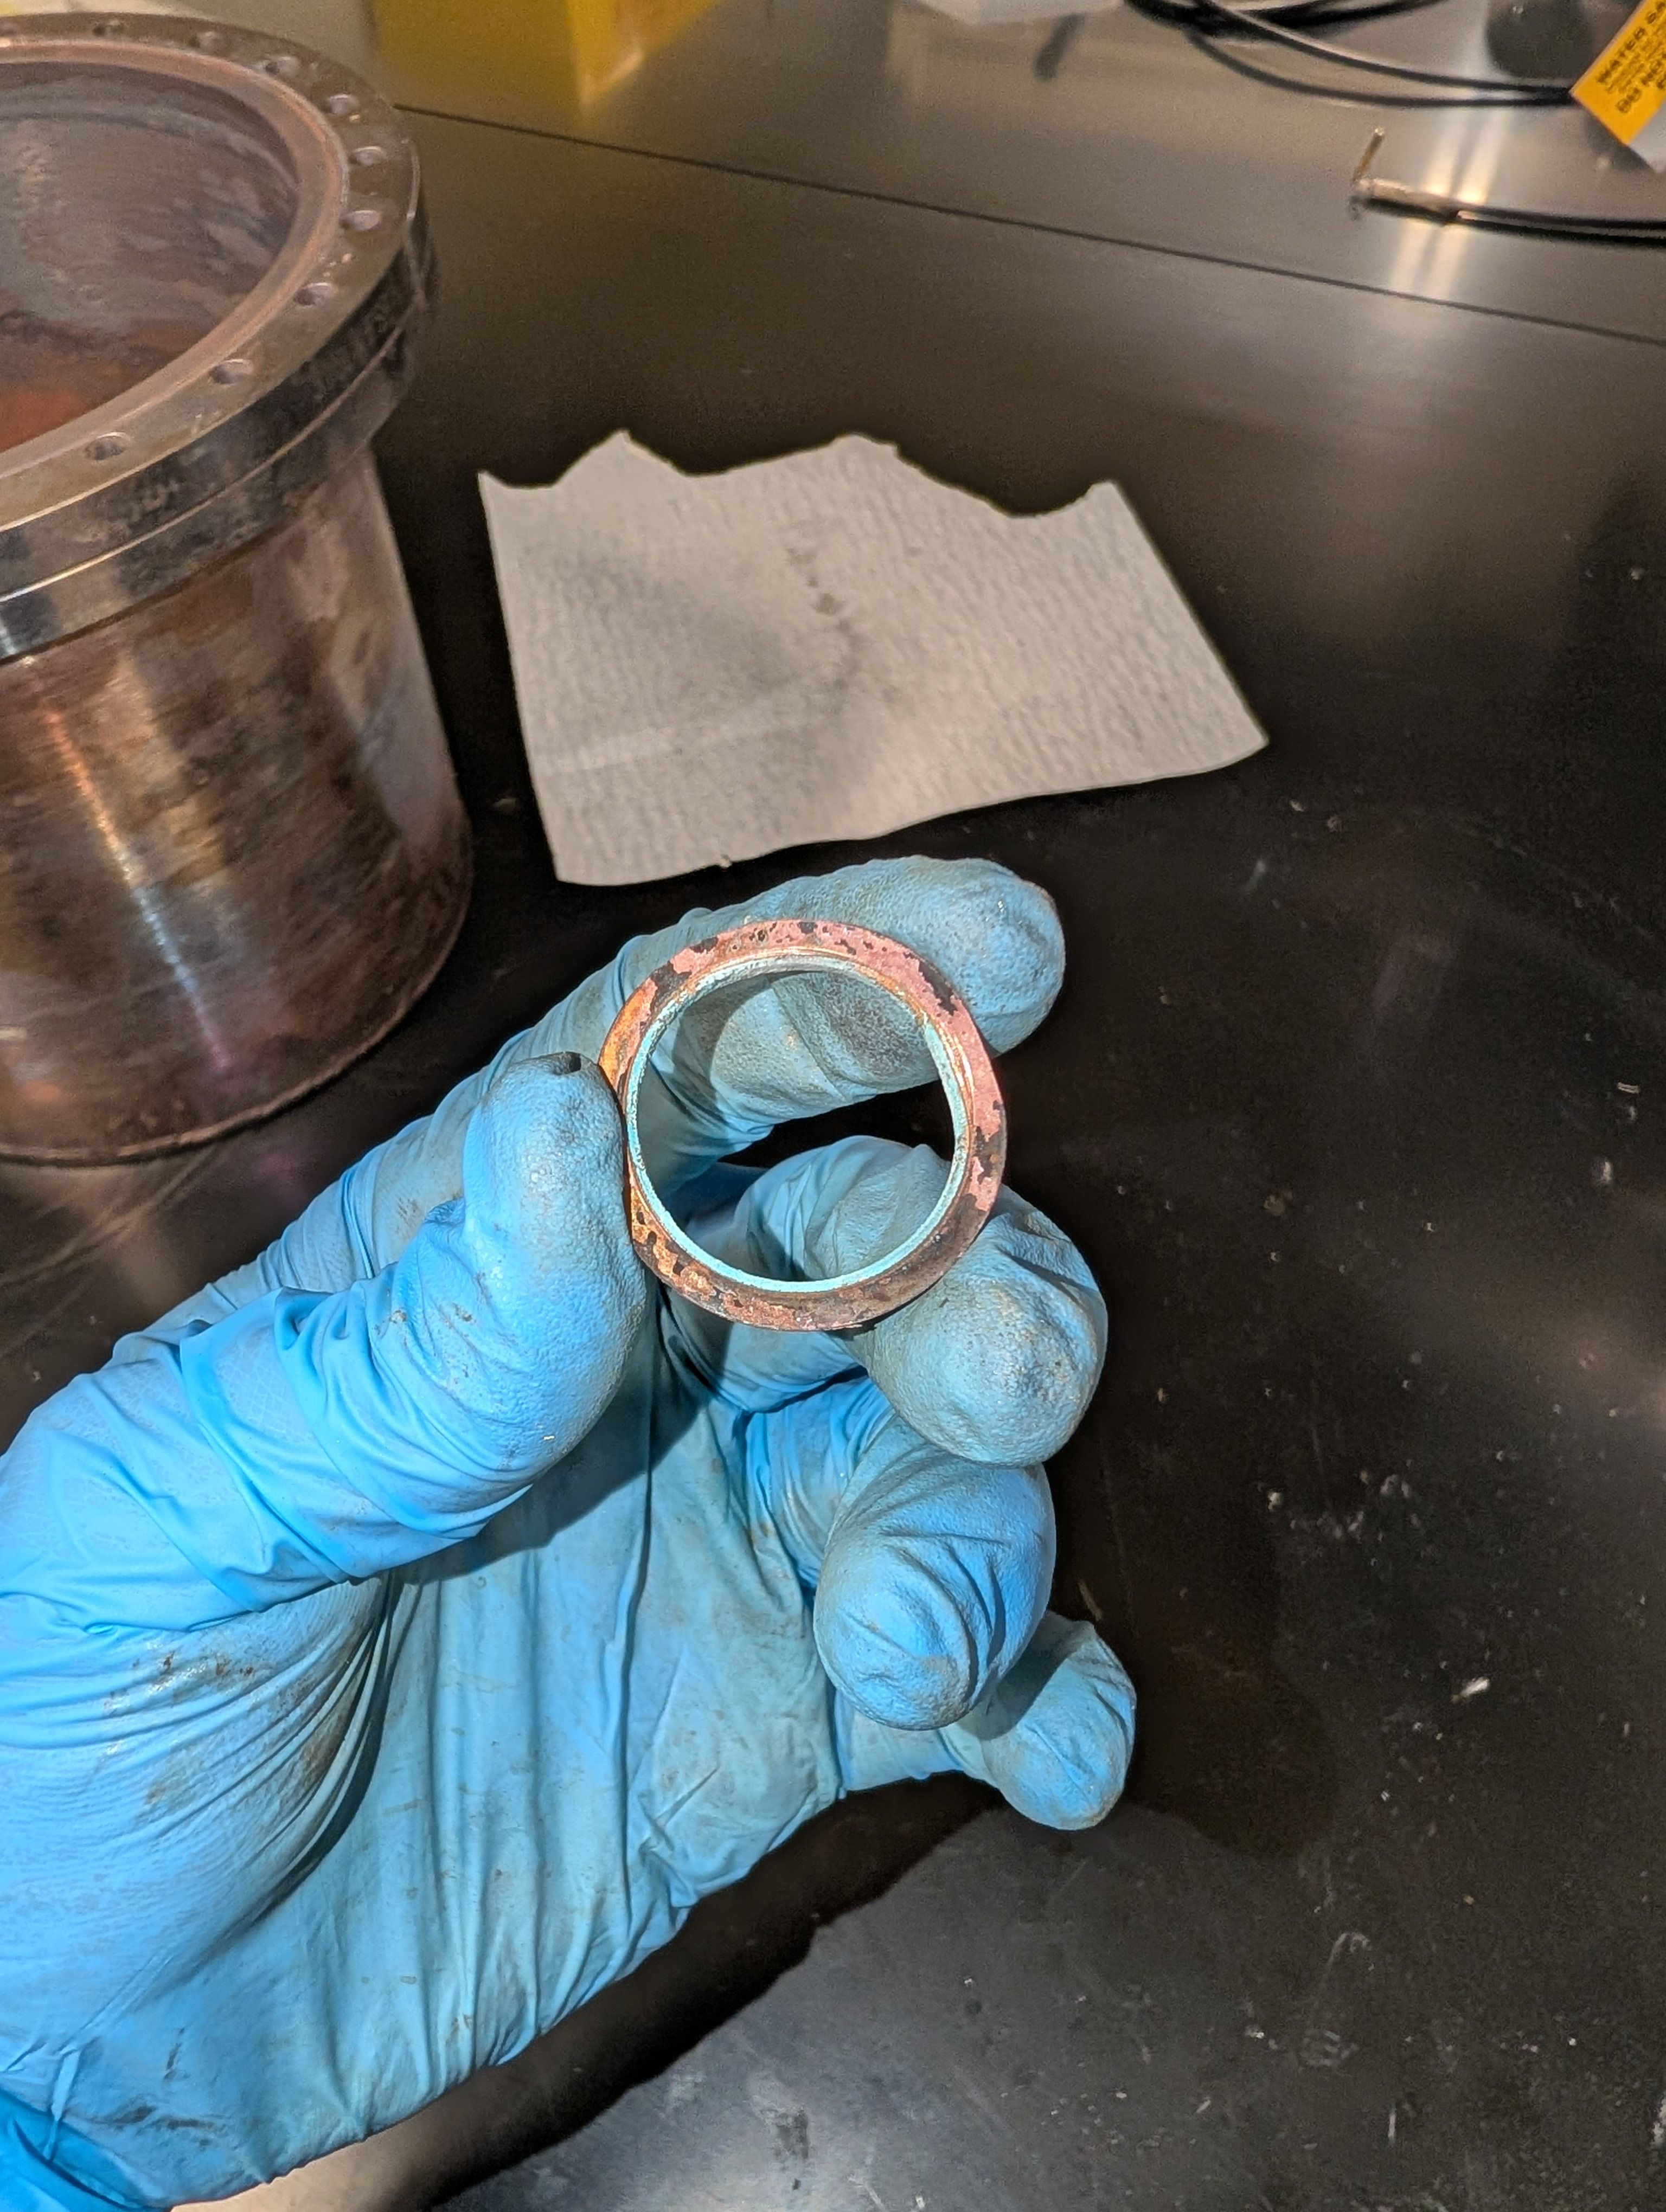
\includegraphics[width=0.6\textwidth]{./assets/pictures/salt feed gasket.jpg}
  \caption{View of the copper gasket on the salt feed port. Note there is
  much less corrosion here than in the chamber lid gasket. (01-16-2026)}
  \label{fig:salt feed gasket}
\end{figure}

\begin{figure}[H]
  \centering
  \includegraphics[width=0.6\textwidth]{./assets/pictures/vacuum pump
  mist filter corrosion.jpg}
  \caption{View of the vacuum pump exhaust port. The pump was used to
    pump corrosive gases, which resulted in
  some corrosion here. (01-22-2026)}
  \label{fig:vacuum pump mist vilter corrosion}
\end{figure}

% TODO: These are scratch notes, incorperate these into the
% document when ready.
Notes on initial cleanup efforts of the FLiNaK purifier. This is
following a containment breach
which resulted in the destruction of the gas bubbler line, as well as
the salt transfer line.
\begin{enumerate}
  \item The reaction chamber was removed from the furnace and
    transferred to the
    glovebox. The transfer tank was also transferred to the glovebox.
  \item The lid was removed from the reaction chamber, along with the
    liner. The 316L stainless steel
    bolts that held the lid together were rusted severely, and many
    bolts were seized. An impact wrench was
    required to loosen the bolts, and a few bolts sheared. The
    transfer tank bolts were similarly corroded and
    seized.
  \item  The Ni liner and lid were stuck together, as the salt dip
    tubes were stuck in the
    frozen salt. Hammering and other mechanical agitation did not
    free the tubes.
  \item To free the dip tubes from the salt, the liner and lid were
    extracted from the argon glovebox and placed inside
    the fumehood furance. The furance was then heated to
    \SI{600}{\celsius} for \SI{2}{\hour}. However, this did not
    melt the FLiNaK.
  \item The temperature was then increased to \SI{700}{\celsius} for
    another hour.
    This melted the FLiNaK, and it was noted that the HF sensor in
    the fume hood registererd
    \qtyrange{1}{2}{ppm}. This was likely due to the FLiNaK reacting
    with water in the air, producing HF and setting off the sensor.
  \item With full PPE, including nitrile + fiber glass heat gloves, a
    labcoat, and a
    full-face HF respirator, the lid was lifted off the liner and
    removed. The furance was then turned off and
    allowed to cool. The room was cleared before and after the
    melting/cooling operation, ensuring that
    nobody was in the vicinity of the fumehood while the HF sensor
    registered the presence of HF.
  \item From a safety perspective, this operation was controlled but
    not ideal. The fumehood where the
    purifier is housed is not rated to handle HF, and does not have
    an acid washdown system.
  \item The reaction chamber and transfer tank were scrubbed with
    water to remove residual FLiNaK and make the system safe for transport
    out of the Houston building where the system operates. Appropriate PPE was
    worn (nitrile gloves, and HF respirator)
  \item The system was transported to the NEEB and disassembled. A
    fractured portion of the salt
    transfer line was cut off of the transfer tank using a reciprocating saw.

    \begin{figure}[H]
      \centering
      \includegraphics[width=0.6\textwidth]{./assets/pictures/damaged
      transfer tank line removed.jpg}
      \caption{The transfer tank with the central salt transfer line cut off.}
      \label{fig: transfer tank damaged line removed}
    \end{figure}

  \item It was noted that the salt dip tubes showed significant
    corrosion. It also appears that salt
    caused Ni to dissolve and redeposited onto the dip tubes,
    resulting in crystalline-like growth on
    the salt tubes. It shold be noted that these tubes were exposed
    to hundreds of hours of
    FLiNaK exposure, many of those hours in the presence of \ch{HF},
    \ch{H2}, and \ch{Ar} gas.
  \item The gas dip tube was ruptured in the stem area. This may have
    allowed for air to enter the system, and would have
    prevented purifier gas from properly bubbling through the salt.

    \begin{figure}[H]
      \centering
      \includegraphics[width=0.6\textwidth]{./assets/pictures/gas
      tube rupture.jpg}
      \caption{A closeup of the lower rupture in the gas bubbler line.}
      \label{fig: gas tube rupture}
    \end{figure}

  \item The reaction chamber and transfer tank were sand-blasted with
    aluminum oxide sandblasting medium at 120 psi to expose fresh surfaces
    and remove remaining salt.
    % TODO: Do this. \item The sandblasting media was then marked as
    % "FLiNaK contaminated" and
    %     appropriate disposal will be done through EHS.
\end{enumerate}
\pagebreak
